%%%%%%%%%%%%%%%%%%%%%%%%%%%%%%%%%%%%%%%%%
% Short Sectioned Assignment LaTeX Template Version 1.0 (5/5/12)
% This template has been downloaded from: http://www.LaTeXTemplates.com
% Original author:  Frits Wenneker (http://www.howtotex.com)
% License: CC BY-NC-SA 3.0 (http://creativecommons.org/licenses/by-nc-sa/3.0/)
%%%%%%%%%%%%%%%%%%%%%%%%%%%%%%%%%%%%%%%%%

%----------------------------------------------------------------------------------------
%	PACKAGES AND OTHER DOCUMENT CONFIGURATIONS
%----------------------------------------------------------------------------------------

\documentclass[paper=a4, fontsize=11pt]{scrartcl} % A4 paper and 11pt font size

% ---- Entrada y salida de texto -----

\usepackage[T1]{fontenc} % Use 8-bit encoding that has 256 glyphs
\usepackage[utf8]{inputenc}
%\usepackage{fourier} % Use the Adobe Utopia font for the document - comment this line to return to the LaTeX default

% ---- Idioma --------

\usepackage[spanish, es-tabla]{babel} % Selecciona el español para palabras introducidas automáticamente, p.ej. "septiembre" en la fecha y especifica que se use la palabra Tabla en vez de Cuadro

% ---- Otros paquetes ----

\usepackage{url} % ,href} %para incluir URLs e hipervínculos dentro del texto (aunque hay que instalar href)
\usepackage{amsmath,amsfonts,amsthm} % Math packages
%\usepackage{graphics,graphicx, floatrow} %para incluir imágenes y notas en las imágenes
\usepackage{graphics,graphicx, float, subfig} %para incluir imágenes y colocarlas

% Para hacer tablas comlejas
%\usepackage{multirow}
%\usepackage{threeparttable}

%\usepackage{sectsty} % Allows customizing section commands
%\allsectionsfont{\centering \normalfont\scshape} % Make all sections centered, the default font and small caps

\usepackage{fancyhdr} % Custom headers and footers
\pagestyle{fancyplain} % Makes all pages in the document conform to the custom headers and footers
\usepackage{eurosym} % Para poder añadir el símbolo del euro
\fancyhead{} % No page header - if you want one, create it in the same way as the footers below
\fancyfoot[L]{} % Empty left footer
\fancyfoot[C]{} % Empty center footer
\fancyfoot[R]{\thepage} % Page numbering for right footer
\renewcommand{\headrulewidth}{0pt} % Remove header underlines
\renewcommand{\footrulewidth}{0pt} % Remove footer underlines
\setlength{\headheight}{13.6pt} % Customize the height of the header

\numberwithin{equation}{section} % Number equations within sections (i.e. 1.1, 1.2, 2.1, 2.2 instead of 1, 2, 3, 4)
\numberwithin{figure}{section} % Number figures within sections (i.e. 1.1, 1.2, 2.1, 2.2 instead of 1, 2, 3, 4)
\numberwithin{table}{section} % Number tables within sections (i.e. 1.1, 1.2, 2.1, 2.2 instead of 1, 2, 3, 4)

\setlength\parindent{0pt} % Removes all indentation from paragraphs - comment this line for an assignment with lots of text

\newcommand{\horrule}[1]{\rule{\linewidth}{#1}} % Create horizontal rule command with 1 argument of height
  % Configuración del documento

%----------------------------------------------------------------------------------------
%	TÍTULO Y DATOS DE LOS ALUMNOS
%----------------------------------------------------------------------------------------

\title{	
	\normalfont \normalsize 
	\textsc{\textbf{Inteligencia de Negocio (2019-2020)} \\ Doble grado en Informática y Matemáticas \\ Universidad de Granada} \\ [25pt] 
	\horrule{0.5pt} \\[0.4cm]
	\huge Práctica 1: Análisis Predictivo Mediante Clasificación usando KNIME \\ 
	\horrule{2pt} \\[0.5cm] 
}

\author{Alberto Jesús Durán López \\
	
		DNI: 54142189 \\
	    Email: albduranlopez@gmail.com \\
         Grupo de prácticas: Martes} 
\date{\normalsize\today}

%----------------------------------------------------------------------------------------
% DOCUMENTO
%----------------------------------------------------------------------------------------

\begin{document}
	\maketitle       % título
	\newpage 
	\tableofcontents % índice
	\newpage
	
	
	
	
	\section{Introducción}
	
	 \hspace{1cm}  En esta práctica veremos el uso de algoritmos de aprendizaje supervisado de clasificación, donde realizaremos un análisis exhaustivo sobre un problema y datos reales, Detección de Fallos en Bombas de Agua en Tanzania. El objetivo es predecir qué bombas de extracción funcionan, cuales no y cuáles necesitan alguna reparación. Los datos con los que trabajamos constan de 39 variables (numéricas y categóricas) y con un total de 59400 instancias). 
	Podemos encontrar este dataset en la página web de la asignatura: \href{url}{http://sci2s.ugr.es/graduateCourses/in} \\
	
	Para entrar en contexto, filtrando la latitud/longitud y pasándola a su coordenada correspondiente, podemos representar (cogiendo una muestra pequeña) la ubicación de las bombas de agua. Claramente es imposible representar el conjunto total de estas, pero modificando un poco los datos de entrada y quedándonos con una pequeña muestra aleatoria generamos la siguiente imagen representativa:
	
	
	\begin{figure}[H]
		\centering
		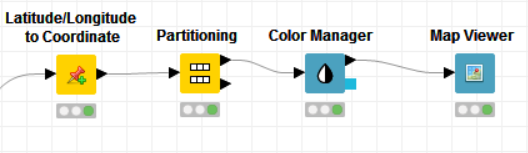
\includegraphics[width=0.6\textwidth]{img/mapa.png}
		\caption{Map Viewer}
	\end{figure}
	
	\begin{figure}[H]
		\centering
		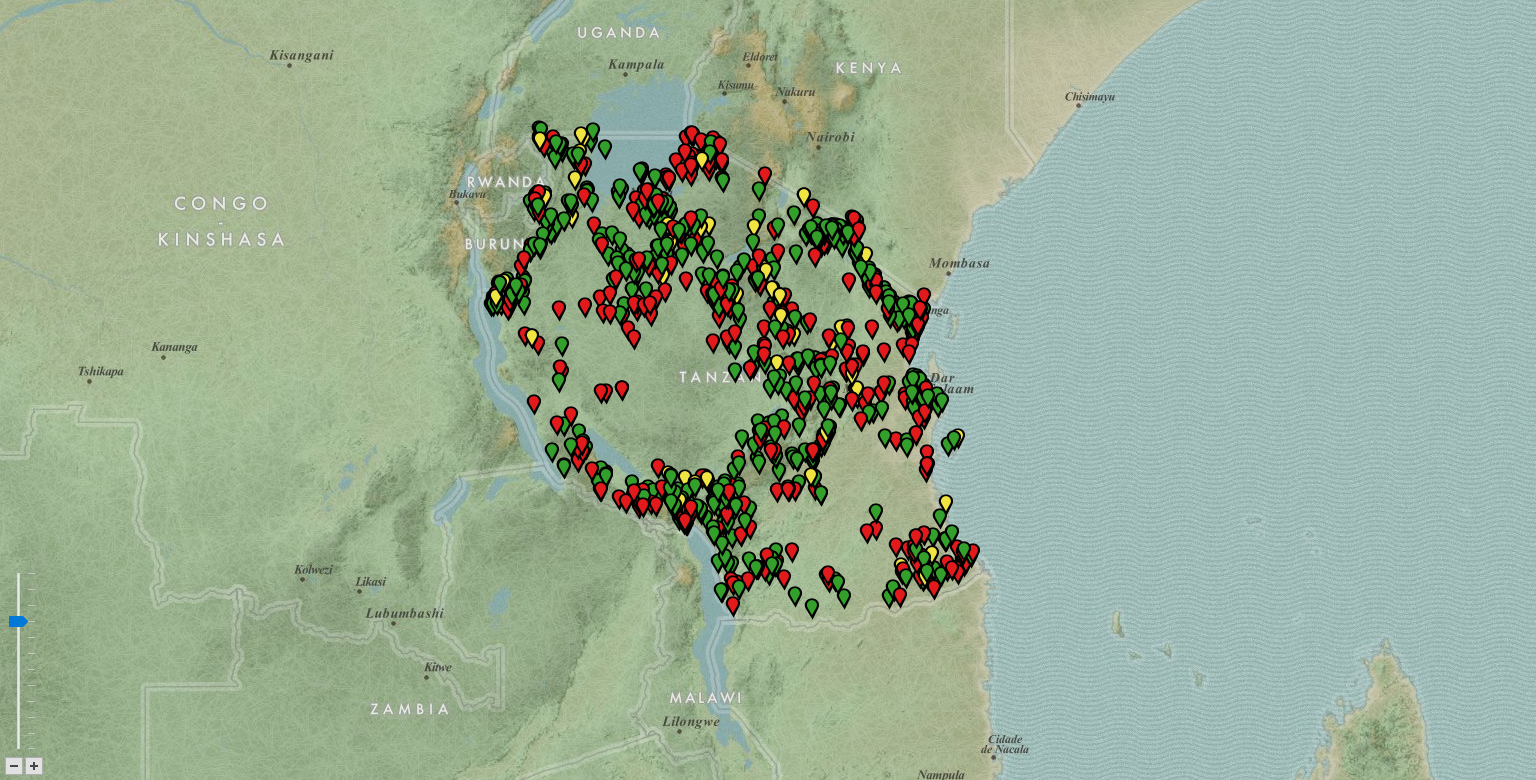
\includegraphics[width=1\textwidth]{img/pump.png}
		\caption{Verde: Functional, Rojas: Non functional, Amarillas: Functional needs repair}
	\end{figure}
	


	\newpage
	

	Se han realizado un total de unas 40 ejecuciones de distintos algoritmos, con modificaciones incluídas. Además, para la visualización de los resultados se han usado gráficas para ayudar su comprensión. El workflout principal es el siguiente:
	
	\begin{figure}[H]
		\centering
		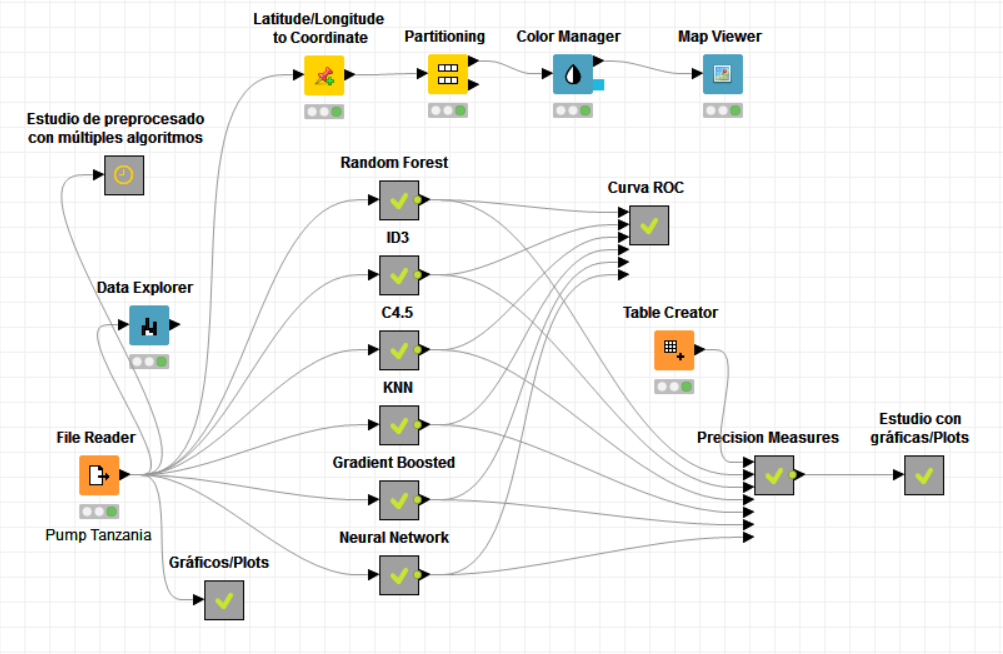
\includegraphics[width=1\textwidth]{img/primer.png}
		\caption{Workflout principal}
	\end{figure}

	En él, hemos encapsulado todos los nodos relacionados. Se ha creado un metanodo para cada algoritmo usado que contendrá numerosos algoritmos y gráficas en su interior.
	
	Por otro lado, se ha creado un metanodo dedicado para el preprocesado y otro para estudiar los datos de entrada iniciales.

	
		
	

	\newpage
	\section{Resultados obtenidos}
	\hspace{1cm} A continuación, se detallarán los diferentes algoritmos usados para abordar el problema así como una breve explicación de cada uno junto a su flujo de trabajo y tablas correspondientes.
	
	Cabe destacar que haremos uso de la técnica \textit{cross-validation} o validación cruzada, en la cual se evalúan los resultados y se garantiza la independencia de la partición entre los datos de entrenamiento y los de prueba.
	
	
	\begin{figure}[H]
		\centering
		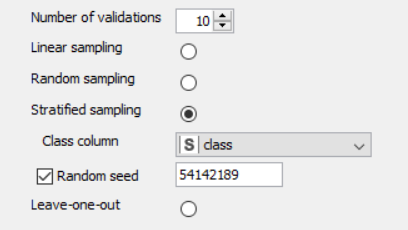
\includegraphics[width=0.5\textwidth]{img/Xrandom.png}
		\caption{X-Partitioner}
	\end{figure}
	
	En dicho nodo, elegimos un total de 10 particiones, con stratified sampling para mantener la proporción de clases del conjunto original y con una semilla aleatoria igual en todos los algoritmos. 
	
	
	\subsection{Random Forest}
	\hspace{1cm} Se trata de una técnica de aprendizaje automático nacida como una mejora de los árboles simples. En este método, se combina una cantidad grande de árboles de decisión independientes, probados sobre conjuntos de datos aleatorios con igual distribución, que se caracteriza principalmente por su estabilidad.
	
	
	\begin{figure}[H]
	    \centering
		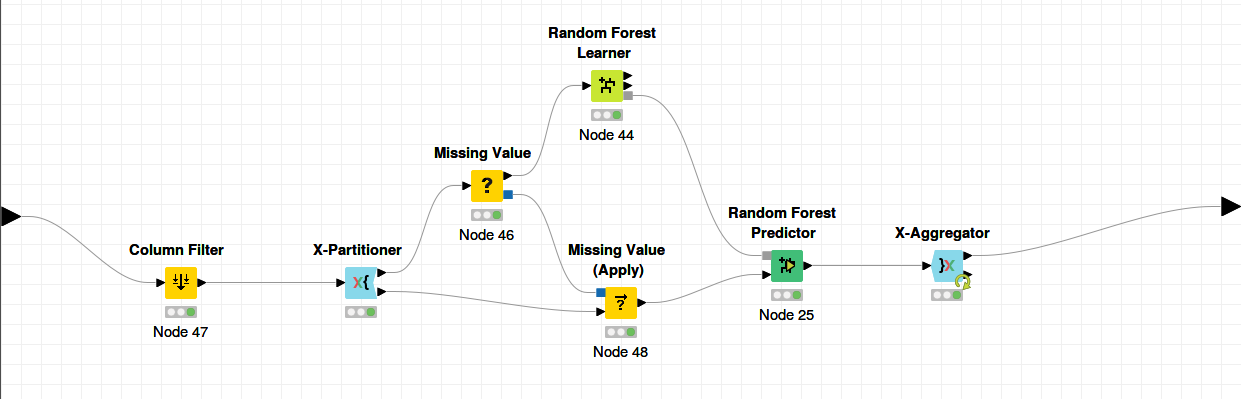
\includegraphics[width=1\textwidth]{img/randomforest.png}
		\caption{Flujo de trabajo. Random Forest}
	\end{figure}

	
	Mostramos el flujo del algoritmo en cuestión. Primeramente hacemos un filtrado de columnas acompañado de X-Partitioner, nodo donde configuramos la validación cruzada, tal y como se muestra en la figura del principio. 
	
	Además, calculamos los valores perdidos usando el nodo \textit{Missing Values} y su \textit{apply} posterior. El criterio de división usado en el nodo \textit{Random Forest Learner} es el de Gini Index con una profundidad máxima de 8 niveles, para así reducir el tiempo de ejecución. En las modificaciones posteriores se alterarán dichos parámetros para intentar mejorar el modelo.
	
	Tras el flujo de trabajo explicado, todo incluido en el mismo metanodo, procedemos a mostrar los resultados. Para esto, hemos creado un metanodo llamado \textit{Precision measures} en el cual se recibe como entrada los algoritmos y se obtiene una tabla comparativa de todos estos. Sin embargo, podemos acceder a los resultados individuales de cada algoritmo:
	
	\begin{figure}[H]
		\centering
		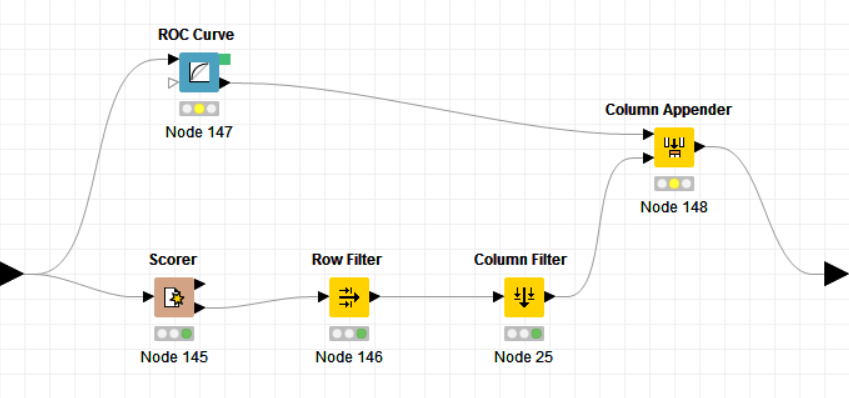
\includegraphics[width=0.8\textwidth]{img/resultados.png}
		\caption{Scorer y Curva ROC individual}
	\end{figure}
	
	Cabe destacar que el Accuracy usado para comparar los algoritmos lo obtenemos a través de \textit{Math Formula}, no del scorer.
	
	Como salida de esta captura anterior tenemos una fila con los valores de los parámetros estudiados: Precision, Sensitivity, Specifity, F-measure, así como el área bajo la curva ROC, obtenida con el nodo \textit{ROC Curve}, que veremos más adelante. Además, la tabla final resultante muestra otros índices, la precisión o \textbf{Accuracy} y la media geométrica o \textbf{G-Mean}.
	
	                                        
	
	\begin{table}[h]
		\resizebox{\textwidth}{!}{%
			\begin{tabular}{|l|l|l|l|l|l|l|l|l|l|l|l|}
				\hline
				\textbf{Algoritmo}        & \textbf{TP} & \textbf{FP} & \textbf{TN} & \textbf{FN} & \textbf{TPR} & \textbf{TNR} & \textbf{PPV} & \textbf{Accuracy} & \textbf{F1-Score} & \textbf{G-mean} & \textbf{AUC} \\ \hline
				\textbf{Random Forest} & 12942       & 1747        & 34829       & 9882        & 0.567        & 0.952        & 0.881        & 0.804             & 0.69              & 0.735           & 0.843                     \\ \hline
			\end{tabular}%
		}
	\end{table}
	
	Por último, comprobaremos el sobreajuste (\textit{Overfitting}) de nuestros algoritmos.
	
	En aprendizaje Automático, el sobreaujuste es el efecto de sobreentrenar un algoritmo de aprendizaje con unos ciertos datos para los que se conoce el resultado.
	
	 Cuando entrenamos nuestro modelo, intentamos \textit{encajar} el conocimiento que pretendemos que adquieran pero puede darse el caso en el que ante nuevas situaciones nuestro modelo no sepa reconocer la muestra con las características aprendidas. \\
	
	Para realizar esto, utilizaremos un nuevo nodo Predictor en cada uno de los algoritmos. Uno de los predictores recibirá los datos del training y el otro los datos del test, tal y como se muestra a continuación:
	
	\begin{figure}[H]
		\centering
		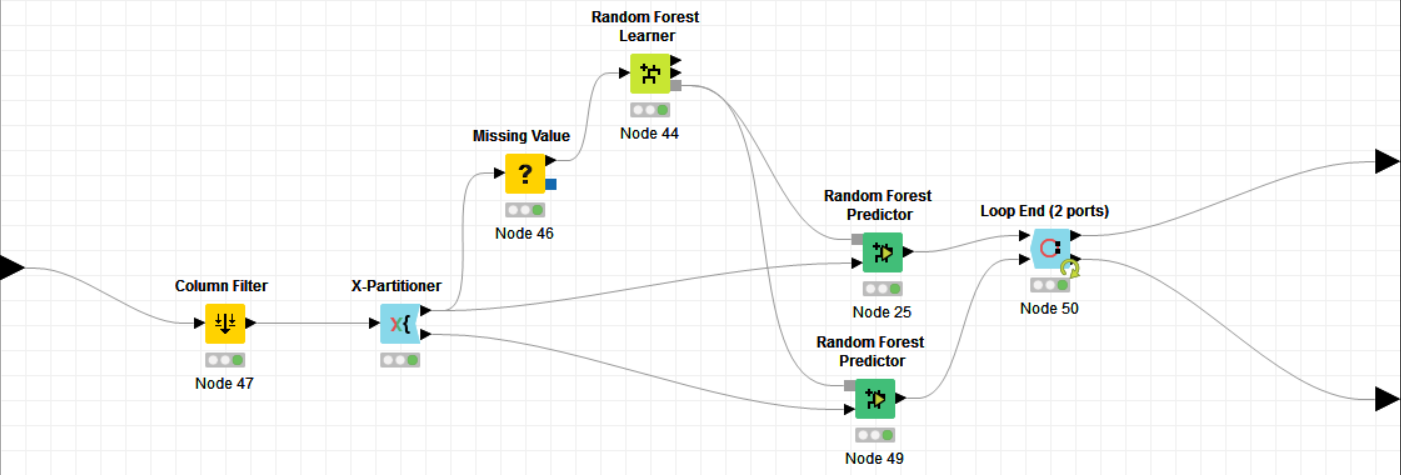
\includegraphics[width=1\textwidth]{img/rfover.png}
		\caption{Resultados}
	\end{figure}

	Los resultados del Overfitting se dejarán y mostrarán en la sección 4.
	
	\subsection{ID3}
	\hspace{1cm} ID3 \textit{Induction Decision Trees}, utilizado en el ámbito de la inteligencia artificial, es un algoritmo que construye un árbol de decisión seleccionando el atributo más útil en cada paso.
	
	\begin{figure}[H]
		    \centering
			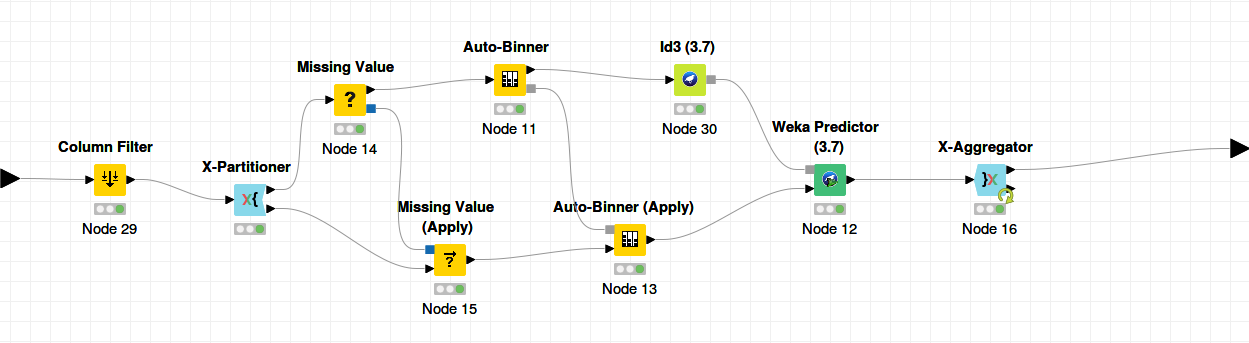
\includegraphics[width=1\textwidth]{img/ID3.png}
			\caption{Flujo de trabajo. ID3}
		\end{figure}
	
	En la imagen anterior se muestra el flujo de trabajo del algoritmo ID3. La estructura del flujo de trabajo es similar al del resto de algoritmos, con la diferencia de que usamos el nodo \textit{autobinner}, que agrupa los datos numéricos en intervalos llamados \textit{bins}.
	
	
	La configuración del nodo ID3 es la que viene por defecto, pues no se puede realizar ninguna modificación. Sin embargo, más adelante realizaremos un preprocesado para compararlos.
	
	\begin{table}[h]
		\resizebox{\textwidth}{!}{%
			\begin{tabular}{|l|l|l|l|l|l|l|l|l|l|l|l|}
				\hline
				\textbf{Algoritmo} & \textbf{TP} & \textbf{FP} & \textbf{TN} & \textbf{FN} & \textbf{TPR} & \textbf{TNR} & \textbf{PPV} & \textbf{Accuracy} & \textbf{F1-Score} & \textbf{G-mean} & \textbf{AUC} \\ \hline
				\textbf{ID3}    & 15995       & 3694        & 32882       & 6829        & 0.701        & 0.899        & 0.812        & 0.823             & 0.752             & 0.794           & 0.853                     \\ \hline
			\end{tabular}
		}
	\end{table}

	\newpage
	
	El flujo de trabajo para comprobar el Overfitting de nuestro algoritmo es el siguiente:
	
	\begin{figure}[H]
		\centering
		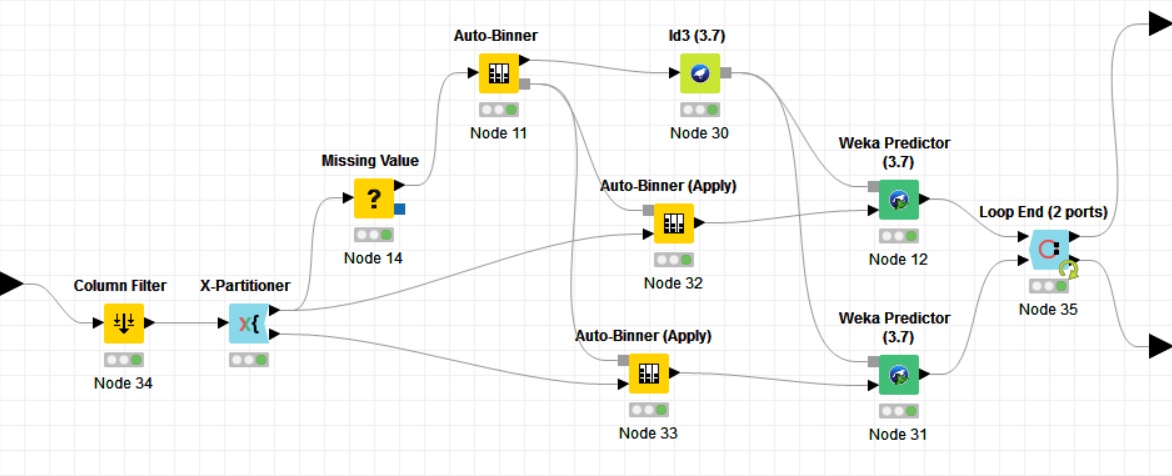
\includegraphics[width=1\textwidth]{img/id3over.png}
		\caption{Overfitting ID3}
	\end{figure}

	En este se vuelven a usar 2 nodos predictores. A uno se le pasan los datos del training y a otro los del test.
	
	
	\subsection{C4.5}
	\hspace{1cm} Se trata de una extensión del algoritmo ID3 en el que se contruye árboles de decisión desde un grupo de datos de entrenamiento de la misma forma en que lo hace ID3, pero usando el concepto de entropía de información.
	
	
	\begin{figure}[H]
		\centering
		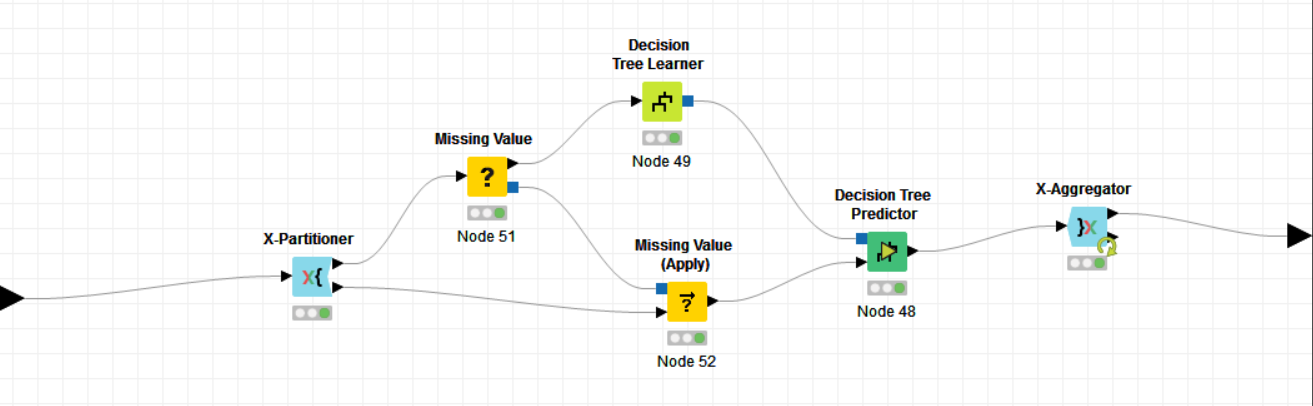
\includegraphics[width=1\textwidth]{img/flujo4.png}
		\caption{Flujo de trabajo. C4.5}
	\end{figure}
	
	
	Flujo de trabajo usando validación cruzada similar al de algoritmos anteriores. Se filtran los datos para rellenar los valores perdidos y en el nodo \textit{Decision Tree Learner}, las opciones configuradas son de 2 registros por nodo (nº mínimo) y 8 hebras, así como Gini Index sin poda.
	
	Tras ejecutar el algoritmo obtenemos los siguientes resultados:
	
	\begin{table}[h]
		\resizebox{\textwidth}{!}{%
			\begin{tabular}{|l|l|l|l|l|l|l|l|l|l|l|l|}
				\hline
				\textbf{Algoritmo} & \textbf{TP} & \textbf{FP} & \textbf{TN} & \textbf{FN} & \textbf{TPR} & \textbf{TNR} & \textbf{PPV} & \textbf{Accuracy} & \textbf{F1-Score} & \textbf{G-mean} & \textbf{AUC} \\ \hline
				\textbf{C4.5}   & 17554       & 4950        & 31324       & 5070        & 0.776        & 0.864        & 0.78         & 0.83              & 0.778             & 0.819           & 0.842                     \\ \hline
			\end{tabular}%
		}
	\end{table}

	Como ejercicio adicional, y ayudándome del siguiente vídeo proporcionado por el profesor de la asignatura \href{url}{https://www.youtube.com/watch?v=H21otPlycA4} , calculamos también el tamaño del árbol. 
	Realmente para un solo algoritmo el tamaño del árbol no aporta información pero como más adelante realizamos diferentes configuraciones con poda o sin ella, se podrán comparar y ver que el tamaño varía sustancialmente.
	
	
	Mostramos a continuación el flujo de trabajo para calcular el tamaño del árbol:
	
	\begin{figure}[H]
		\centering
		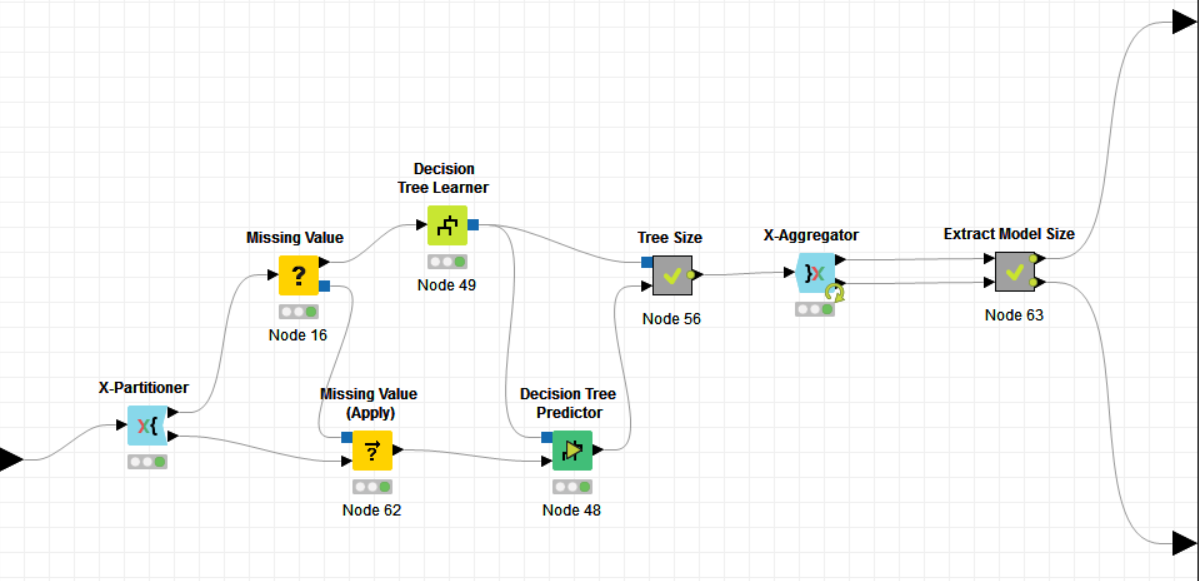
\includegraphics[width=1\textwidth]{img/size.png}
		\caption{Flujo de trabajo - Model Size}
	\end{figure}

	Tal y como se indica en el flujo de trabajo, extraemos el tamaño del árbol y lo incluimos en la tabla de resultados para las modificaciones que realizaremos en  en el apartado 4.
	
	Por último, calculamos el Overfitting del C4.5
	\begin{figure}[H]
		\centering
		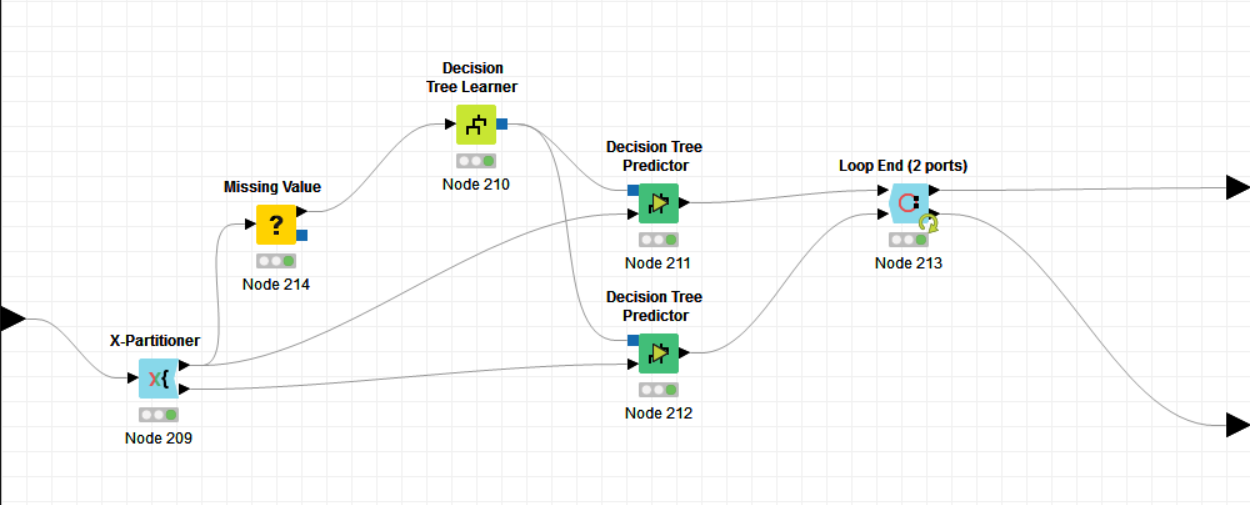
\includegraphics[width=1\textwidth]{img/c45over.png}
		\caption{Overfitting C4.5}
	\end{figure}
	
	
	
	\subsection{KNN}
	\hspace{1cm} Conocido como \textit{K-nearest neighbors}, KNN es un algoritmo de aprendizaje supervisado que se basa en la suposición de que los prototipos más cercanos tienen una probabilidad a posteriori similar. Al igual que pasa con las redes neuronales, KNN solo trabaja con valores numéricos por lo que hay que convertir los datos de entrada. Además, se normalizan para que trabajen en el mismo rango.
	
	
	\begin{figure}[H]
		    \centering
			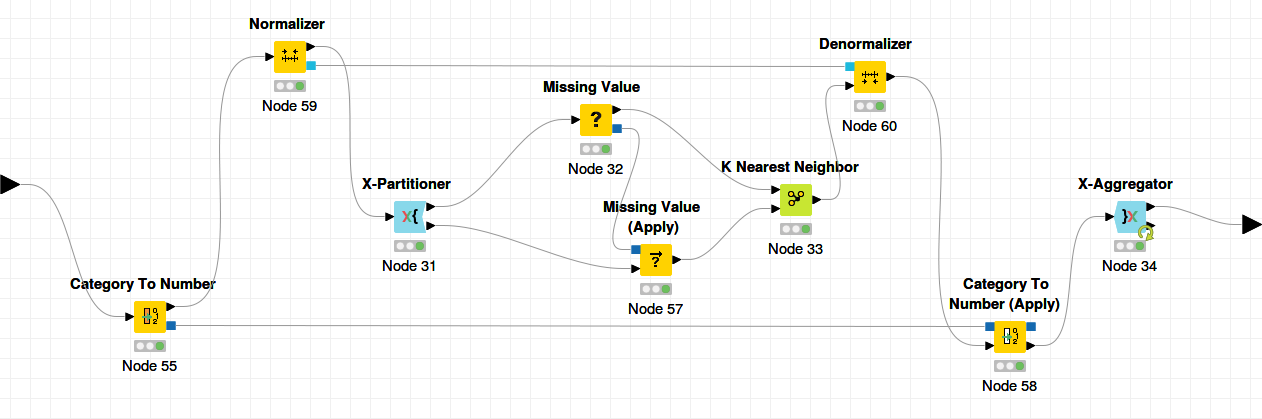
\includegraphics[width=1\textwidth]{img/KNN.png}
			\caption{Flujo de trabajo. KNN}
		\end{figure}
	
	Es un algoritmo supervisado y basado en instancias. 
	
	Además, a diferencia del resto de algoritmos, necesita que los datos de entrada sean valores numéricos. En nuestro dataset tenemos bastantes atributos de tipo string que por una parte se pueden filtrar con \textit{Column Filter} o se pueden convertir.
	En nuestro caso, además de convertirlos, los normalizamos para que así el modelo siga las propiedades de una distribución Normal(0,1), lo que se ve reflejado en unos mejores resultados. 
	
	\begin{table}[h]
		\resizebox{\textwidth}{!}{%
			\begin{tabular}{|l|l|l|l|l|l|l|l|l|l|l|l|}
				\hline
				\textbf{Algoritmo} & \textbf{TP} & \textbf{FP} & \textbf{TN} & \textbf{FN} & \textbf{TPR} & \textbf{TNR} & \textbf{PPV} & \textbf{Accuracy} & \textbf{F1-Score} & \textbf{G-mean} & \textbf{AUC} \\ \hline
				\textbf{KNN}    & 16560       & 5374        & 31202       & 6264        & 0.726        & 0.853        & 0.755        & 0.804             & 0.74              & 0.787           & 0.86                      \\ \hline
			\end{tabular}%
		}
	\end{table}


	El flujo de trabajo siguiente muestra los nodos necesarios para comprobar el Overfitting de KNN:

	\begin{figure}[H]
		\centering
		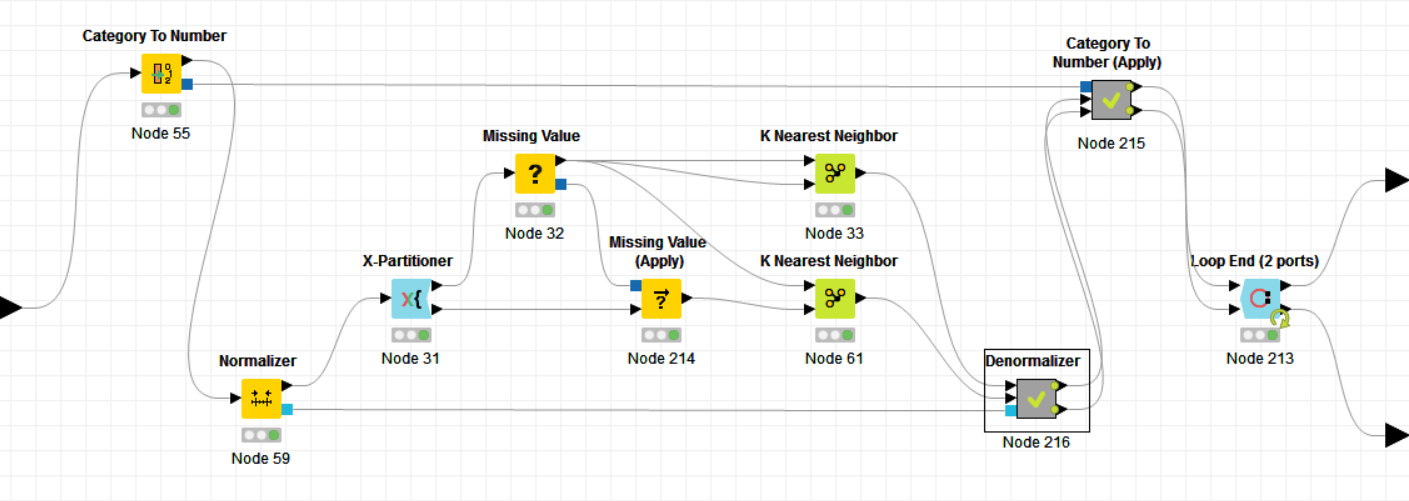
\includegraphics[width=1\textwidth]{img/knnover.png}
		\caption{Overfitting KNN}
	\end{figure}

	Se han creado dos metanodos adicionales donde se desnormaliza y se aplica \textit{Category To Number (Apply)}
	

	\subsection{Gradient Boosted}
	\hspace{1cm} Se trata de una generalización del algoritmo \textit{AdaBoost} caracterizado principalmente por su flexibilidad para aplicar boosting a multitud de problemas y caracterizado por ir minimizando los residuos iteración a iteración.
	
	
	
	\begin{figure}[H]
		    \centering
			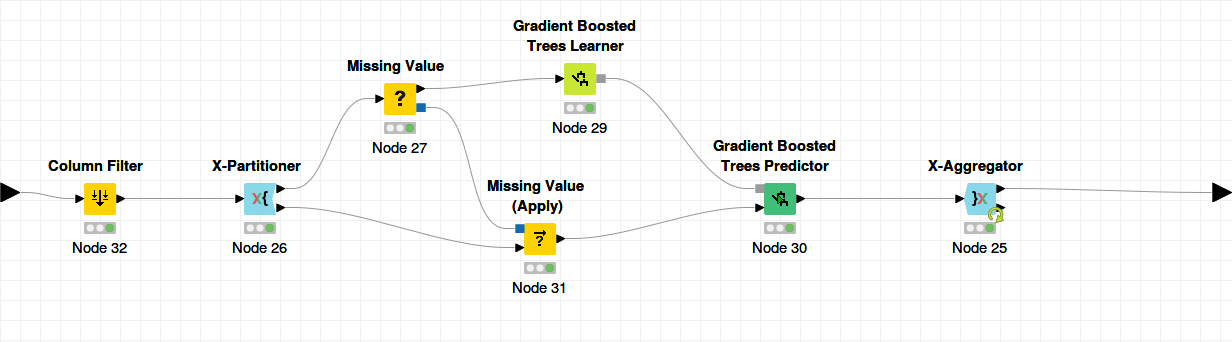
\includegraphics[width=1\textwidth]{img/Gradient.png}
			\caption{Flujo de trabajo. Gradient Boosted}
		\end{figure}
	
	Es quizás el algoritmo que más ha costado tratar por el gran tiempo que tarda en su ejecución. Durante el transcurso de su ejecución se han tenido problemas de espacio en la pila, por lo que hemos tenido que meternos en el archivo de configuración de KNIME y aumentar el espacio de la RAM que se le reservaba al programa. \\
	
	
	Los resultados obtenidos tras su ejecución son los siguientes.
	\begin{table}[h]
		\resizebox{\textwidth}{!}{%
			\begin{tabular}{|l|l|l|l|l|l|l|l|l|l|l|l|}
				\hline
				\textbf{Algoritmo}           & \textbf{TP} & \textbf{FP} & \textbf{TN} & \textbf{FN} & \textbf{TPR} & \textbf{TNR} & \textbf{PPV} & \textbf{Accuracy} & \textbf{F1-Score} & \textbf{G-mean} & \textbf{AUC} \\ \hline
				\textbf{Gradient Boosted} & 13426       & 2287        & 34289       & 9398        & 0.588        & 0.937        & 0.854        & 0.803             & 0.697             & 0.743           & 0.859                     \\ \hline
			\end{tabular}%
		}
	\end{table}
	
	
	La siguiente imagen muestra el flujo de trabajo para calcular el Overfitting de nuestro algoritmo.
	
	\begin{figure}[H]
		\centering
		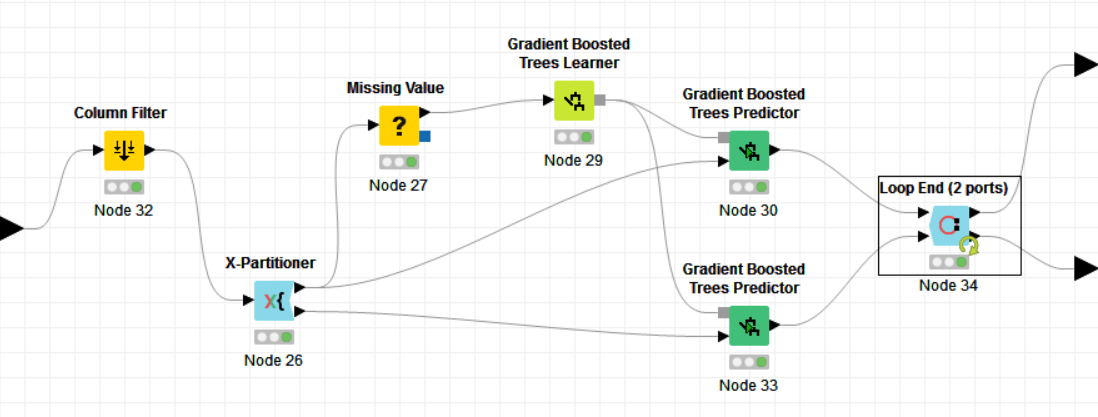
\includegraphics[width=0.8\textwidth]{img/gbover.png}
		\caption{Overfitting Gradient Boosted}
	\end{figure}
	
	\subsection{Neural Network}
	\hspace{1cm} En nuestro caso usaremos \textbf{Perceptrón multicapa, RNA}, formada por múltiples capas, de tal manera que tiene la capacidad de resolver problemas que no son linealmente separables.
	
	Cabe destacar que la red neuronal solo acepta valores numéricos por lo que usando el nodo \textit{Category to Number} convertimos dichos valores. Por otro lado, tenemos muchas columnas con muchos valores numéricos de diferentes rangos. Es por esto por lo que los datos deben estar normalizados, es decir, red neuronal no podría comparar los valores de diferentes órdenes de magnitud.
	Para ello usamos el nodo \textit{Normalizer}.
	\newpage
	
	Mostramos los resultados y el flujo de trabajo de Neural Network: 
	\begin{figure}[H]
		    \centering
			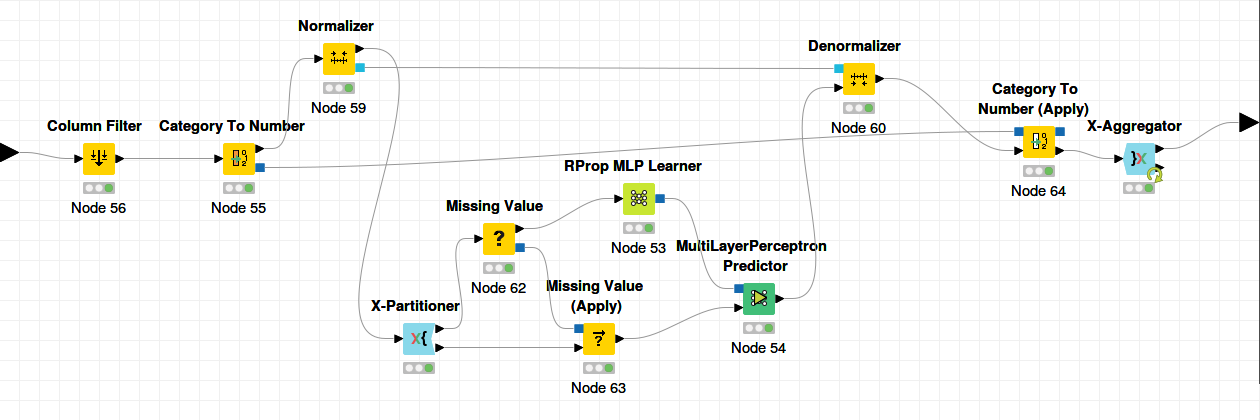
\includegraphics[width=1\textwidth]{img/Neural.png}
			\caption{Flujo de trabajo. Neural Network}
		\end{figure}
	
	Ejecutamos nuestro  algoritmo y obtenemos los siguientes resultados:
	
	\begin{table}[]
		\resizebox{\textwidth}{!}{%
			\begin{tabular}{|l|l|l|l|l|l|l|l|l|l|l|l|}
				\hline
				\textbf{Algoritmo}         & \textbf{TP} & \textbf{FP} & \textbf{TN} & \textbf{FN} & \textbf{TPR} & \textbf{TNR} & \textbf{PPV} & \textbf{Accuracy} & \textbf{F1-Score} & \textbf{G-mean} & \textbf{AUC} \\ \hline
				\textbf{Neural Network} & 14591       & 5087        & 31489       & 8233        & 0.639        & 0.861        & 0.741        & 0.776             & 0.687             & 0.742           & 0.828                     \\ \hline
			\end{tabular}%
		}
	\end{table}

	Con gran diferencia, la red neuronal es el algoritmo que peores resultados produce.

	\section{Análisis de resultados}
	
	\subsection{Índices/Medidas}
	\hspace{1cm} Para entrar en materia, explicaremos qué representan los índices obtenidos en las diferentes tablas de los algoritmos:
	
	\begin{itemize}
		\item \textbf{TP}: True positive.
		\item \textbf{FP}: False positive.
		\item \textbf{TN}: True negative.
		\item \textbf{FN}: False negative.
		
		Estos cuatro valores anteriores se pueden agrupar en lo que se conoce \textbf{Matriz de confusión}.
		
		\begin{figure}[H]
			\centering
			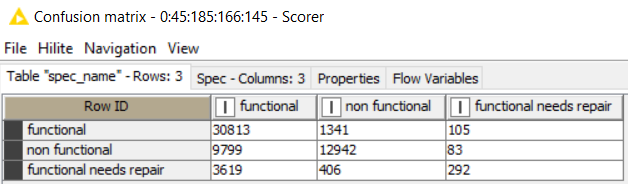
\includegraphics[width=0.8\textwidth]{img/confusion.png}
			\caption{Matriz Confusión Random Forest}
		\end{figure}
		
		\item \textbf{TPR}: True positive rate (Sensitivity)
		
		$TPR=\frac{TP}{TP+FN}$
		\item \textbf{FPR}: False positive rate
		
		$FPR=\frac{FP}{TN+FP}$
		
		\item \textbf{TNR}: True negative rate (Specifity)
		
		$TNR=\frac{TN}{TN+FP}$
		
		\item \textbf{PPV}: Positive predictive values (Precision)
		
		$PPV=\frac{TP}{TP+FP}$
		
		\item \textbf{Accuracy}: Precisión. Medida que divide las predicciones correctas entre el número total de predicciones. Cuando las clases no están balanceadas conviene emplear otras medidas de evaluación que tienen en cuenta la distribución del error entre clases.
		
		$Accuracy=\frac{TP+TN}{TP+FP+TN+FN}$
		
		\item \textbf{F1-Score}: Es la media armónica de PPV y TPR.
		
		$F1=\frac{2TP}{2TP+FP+FN}$


		\item \textbf{G-mean}: Media geométrica
		
		$Gmean=\sqrt{ \frac{TP \cdot TN}{(TP+FN)\cdot(TN+FP)}} = \sqrt{TPR \cdot TNR}$
	
	
		\item \textbf{AUC}: Area Under Curve
		
		$AUC=\frac{1+TPR-FPR}{2}$
	\end{itemize}
	
	
	Concatenamos las tablas de todos los algoritmos y añadimos la medida de la media geométrica y del Área bajo la curva usando \textit{Math Formula}
	
	\begin{figure}[H]
		\centering
		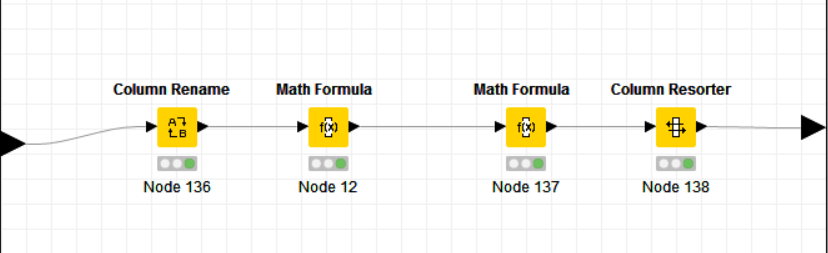
\includegraphics[width=1\textwidth]{img/math.png}
		\caption{Accuracy + G-mean, Math Formula}
	\end{figure}


	\begin{figure}[H]
		\begin{minipage}[b]{0.45\linewidth}
			\centering
			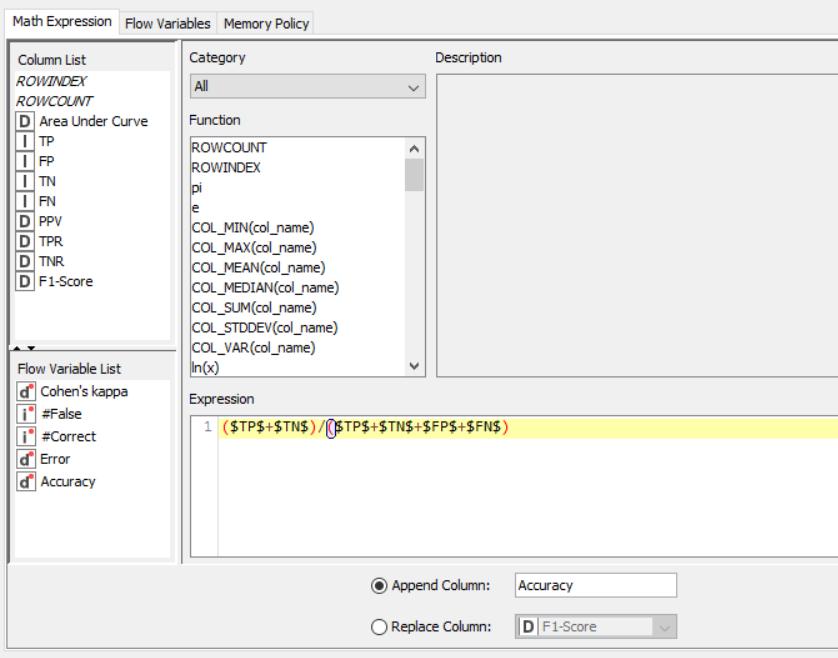
\includegraphics[width=0.9\linewidth]{img/math1.png}
			\caption{Accuracy}
		\end{minipage}
		\hspace{0.5cm}
		\begin{minipage}[b]{0.45\linewidth}
			\centering
			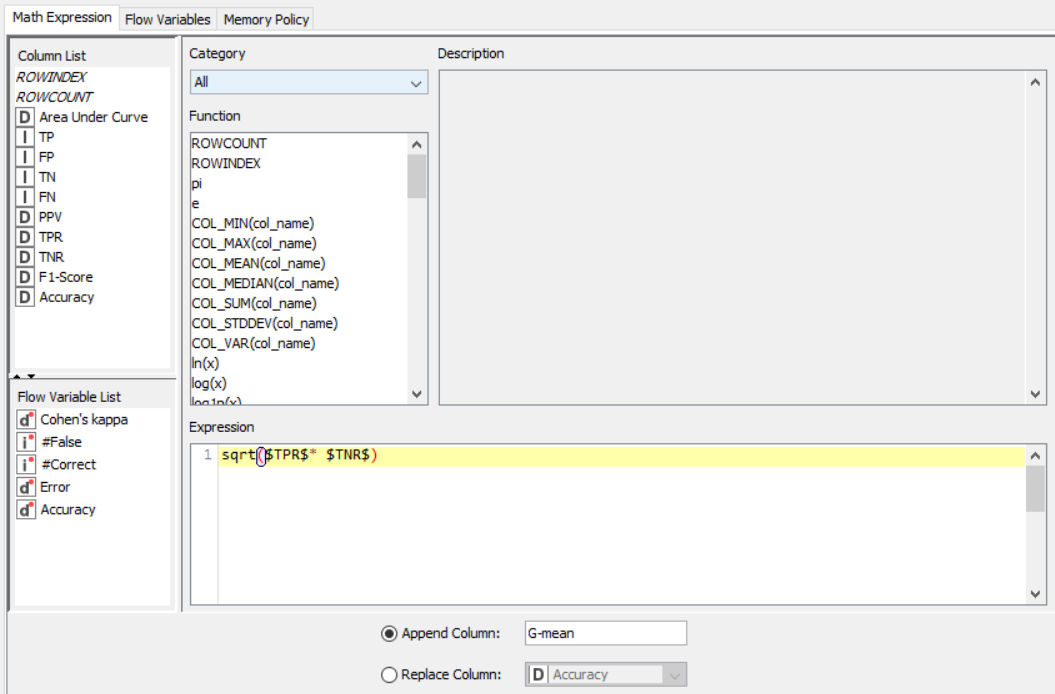
\includegraphics[width=1.1\linewidth]{img/math2.png}
			\caption{G-Mean}
		\end{minipage}
	\end{figure}
	
	
	
	Una vez añadidas las fórmulas de estos índices (y siguiendo el video de youtube del profesor de la asignatura), ejecutamos y mostramos los resultados:
	
	\begin{table}[H]
		\resizebox{\textwidth}{!}{%
			\begin{tabular}{|l|l|l|l|l|l|l|l|l|l|l|l|}
				\hline
				\textbf{Algoritmo}           & \textbf{TP} & \textbf{FP} & \textbf{TN} & \textbf{FN} & \textbf{TPR} & \textbf{TNR} & \textbf{PPV} & \textbf{Accuracy} & \textbf{F1-Score} & \textbf{G-mean} & \textbf{AUC} \\ \hline
				\textbf{Random Forest}    & 12942       & 1747        & 34829       & 9882        & 0.567        & 0.952        & 0.881        & 0.804             & 0.69              & 0.735           & 0.843                     \\ \hline
				\textbf{ID3}              & 15995       & 3694        & 32882       & 6829        & 0.701        & 0.899        & 0.812        & 0.823             & 0.752             & 0.794           & 0.853                     \\ \hline
				\textbf{C4.5}             & 17554       & 4950        & 31324       & 5070        & 0.776        & 0.864        & 0.78         & 0.83              & 0.778             & 0.819           & 0.842                     \\ \hline
				\textbf{KNN}              & 16560       & 5374        & 31202       & 6264        & 0.726        & 0.853        & 0.755        & 0.804             & 0.74              & 0.787           & 0.86                      \\ \hline
				\textbf{Gradient Boosted} & 13426       & 2287        & 34289       & 9398        & 0.588        & 0.937        & 0.854        & 0.803             & 0.697             & 0.743           & 0.859                     \\ \hline
				\textbf{Neural Network}   & 14591       & 5087        & 31489       & 8233        & 0.639        & 0.861        & 0.741        & 0.776             & 0.687             & 0.742           & 0.828                     \\ \hline
			\end{tabular}%
		}
	\end{table}

	En este caso, el algoritmo que tiene mejor Accuracy es el C4.5 con un total de 0.83. Sin embargo, esta medida no se considera buena (como ya hemos explicado antes) si las clases no están balanceadas.
	Si vemos la media geométrica \textbf{G-mean}, el mejor algoritmo sería también C4.5 pero no ocurre por ejemplo si observamos el \textbf{Area Under Curve} donde KNN y Gradient Boosted se llevan la victoria.

	
	\subsection{Bar Chart}
	
	\hspace{1cm} Mostramos ahora los resultados con un diagrama de barras común donde representamos los cuatro principales índices.
	
	\begin{figure}[H]
		\centering
		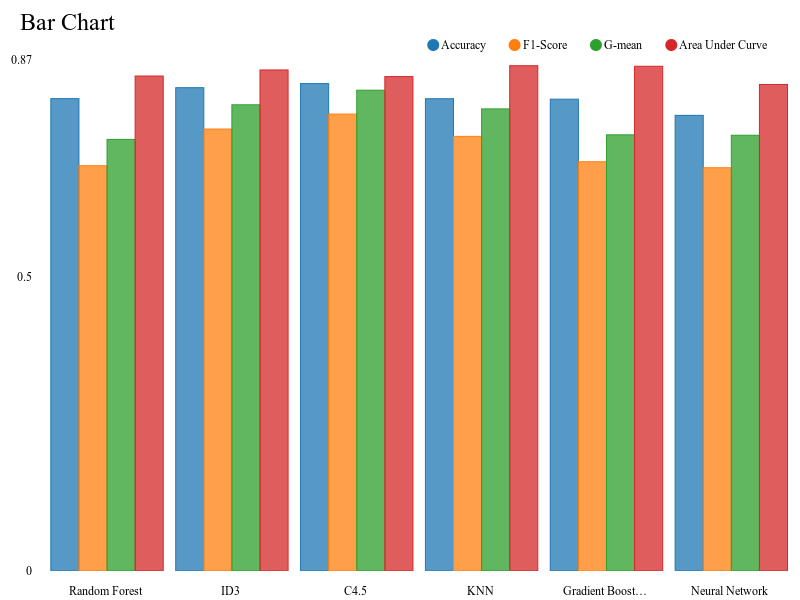
\includegraphics[width=0.65\textwidth]{img/h1.png}
		\caption{Resultados}
	\end{figure}
	
	Observando la gráfica anterior, los resultados parece que son prácticamente iguales. Esto es porque se representa todo el intervalo entero (desde 0 hasta el valor máximo obtenido, 0.87). Es por esto por lo que el diagrama de barras no nos aporta una buena información de cara a una comparación exhaustiva.


	\subsection{Curva ROC/Parallel plot}
	
	\hspace{1cm} Se trata de una representación gráfica de la razón de True Positive Rate (TPR) frente a True Negative Rate (TNR). Representamos todas las curvas ROC unidas en una grupal. Abajo a la derecha tenemos una leyenda que nos índica del color en cuestión seguido de un número que indica el valor de AUC (Area Under Curve)
	
	\begin{figure}[H]
		\centering
		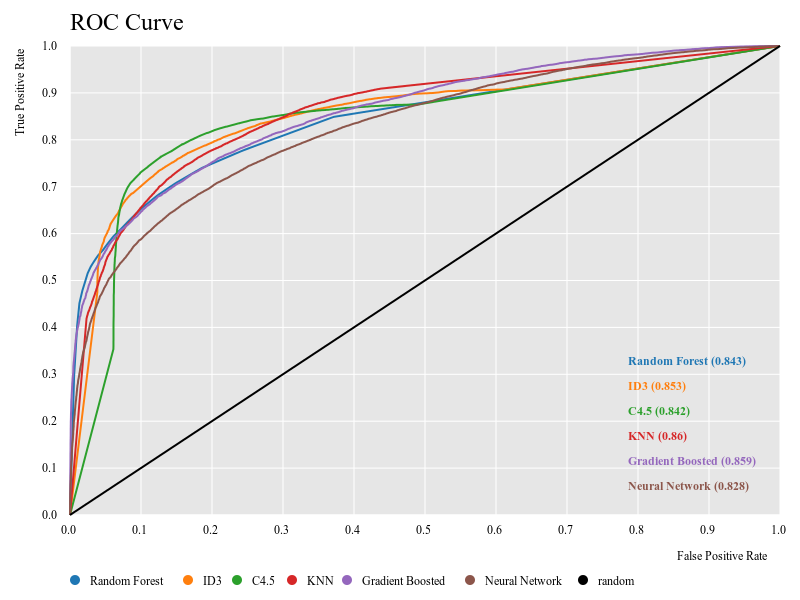
\includegraphics[width=1\textwidth]{img/allroc.png}
		\caption{Curva ROC comparativa}
	\end{figure}


	Todos los algoritmos muestran resultado parecidos. Difieren en las centésimas y el valor medio está en torno a un 0.85 por lo que podemos afirmar que los algoritmos producen buenos resultados. \\

	\newpage 
	Tras probar con diferentes tipos de gráficas, hemos encontrado \textit{Parallel Coordinates Plot}, un gráfico parecido al \textit{Radar Plot} pero con la diferencia de que une todos los algoritmos en una sola tabla. La configuración de este gráfico no admite leyenda por lo que hemos optado por crear una nueva columna llamada Method e incluirla en la representación para no perdernos en la lectura.
	
	\begin{figure}[H]
		\centering
		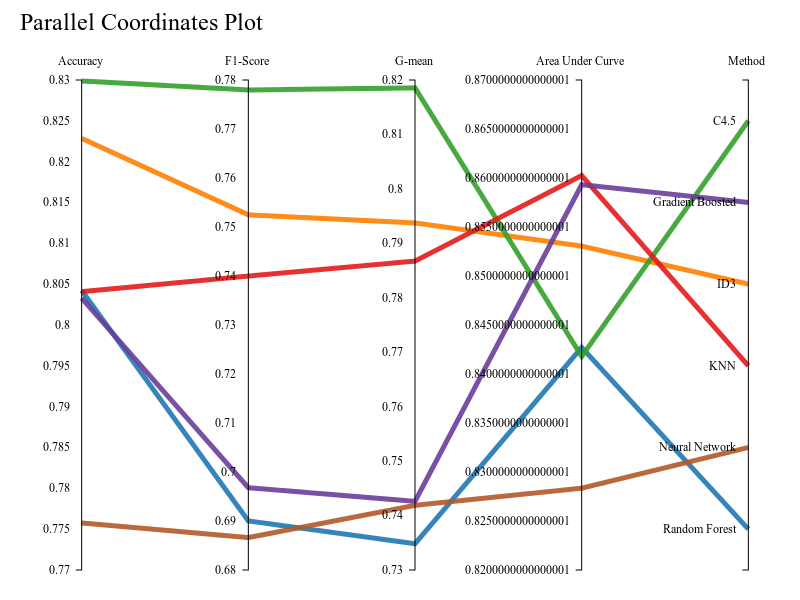
\includegraphics[width=0.8\textwidth]{img/parallel2.png}
		\caption{Resultados}
	\end{figure}

	Tras mostrar los resultados y observando la tabla anterior, todos los índices indican que el algoritmo menos eficiente y que peor clasifica los datos es la Red Neuronal, acompañada de Random Forest. 
	
	El hecho de que las clases no estén balanceadas no es el causante de estos malos resultados. Un factor puede ser el nº de iteracciones seleccionado para su ejecución (200 iteraciones) ya que se puede producir ruido u Overfitting.
	
	Por otro lado, el resto de algoritmos se mantienen en la misma línea. El que consigue un mayor \textbf{Accuracy} es C4.5, aunque baja drásticamente en el índice \textbf{AUC}. 
	
	Observando la expresión de las fórmulas de la precisión y del area bajo la curva, observamos que debe ser porque FPR (False Positive Rate) incrementa, es decir, FP es elevado en dicho algoritmo y al estar en el numerador y restando en la fórmula de Area Under Curve, hace decrementar el valor del índice.
	
	Por último, cabe destacar la monotonía del algoritmo ID3. No presenta picos de subidas ni bajadas por lo que no sería descabellado intentar preprocesarlo y modificarlo y obtener así una buena efectividad.
	


	

	\newpage 
	\section{Configuración de algoritmos}
	\hspace{1cm} Esta sección la dedicaremos a las multiples y diferentes modificaciones realizadas a todos los algoritmos. 
	Para ayudar a la lectura del proyecto, se ha encapsulado cada modificación en un distinto de forma que todos los resultados se unen en una tabla final comparativa en la cual conectaremos diferentes \textit{plots} para su correcta representación.

	
	
	\subsection{Random Forest}
	
	\hspace{1cm} El primer algoritmo a modificar será Random Forest en el cual utilizamos diferentes coeficientes, \textit{Gain Ratio} y \textit{Gini Index}.
	
	\begin{itemize}
		\item \textbf{Gini Index}: mide el grado o la probabilidad de una variable particular siendo erróneamente clasificada cuando se escoge aleatoriamente.
		\item \textbf{Gain Ratio}: es el cociente entre \textit{Information Gain (Ganancoa de información de una variable aleatoria observando otra variable aleatoria) y un valor intrínseco definido para los árboles en Aprendizaje Automático. }
		
	\end{itemize}
	

	\begin{figure}[H]
		\centering
		\includegraphics[width=1\textwidth]{img/rfcomp.png}
		\caption{Workflow Random Forest}
	\end{figure}


	Mostramos en la siguiente tabla los resultados en el cual seleccionamos un total de 8 y 12 hebras combinando los dos índices anteriormente explicados:

	\begin{table}[h]
		\resizebox{\textwidth}{!}{%
			\begin{tabular}{|l|l|l|l|l|l|l|l|l|l|l|l|}
				\hline
				\textbf{Algoritmo}                 & TP    & FP   & TN    & FN    & TPR   & TNR   & PPV   & Accuracy & F1-Score & G-mean & AUC \\ \hline
				\textbf{Random Forest, Gini 8}  & 12942 & 1747 & 34829 & 9882  & 0.567 & 0.952 & 0.881 & 0.804    & 0.69     & 0.735  & 0.843            \\ \hline
				\textbf{Random Forest, Gini 12} & 15018 & 2074 & 34502 & 7806  & 0.658 & 0.943 & 0.879 & 0.834    & 0.752    & 0.788  & 0.887            \\ \hline
				\textbf{Random Forest, Gain 8}  & 11109 & 1356 & 35220 & 11715 & 0.487 & 0.963 & 0.891 & 0.78     & 0.63     & 0.685  & 0.776            \\ \hline
				\textbf{Random Forest, Gain 12} & 11911 & 1348 & 35228 & 10913 & 0.522 & 0.963 & 0.898 & 0.794    & 0.66     & 0.709  & 0.806            \\ \hline
			\end{tabular}%
		}
	\end{table}

	\newpage
	
	Mostramos los resultados en un gráfico de barras:
	

	\begin{figure}[H]
		\centering
		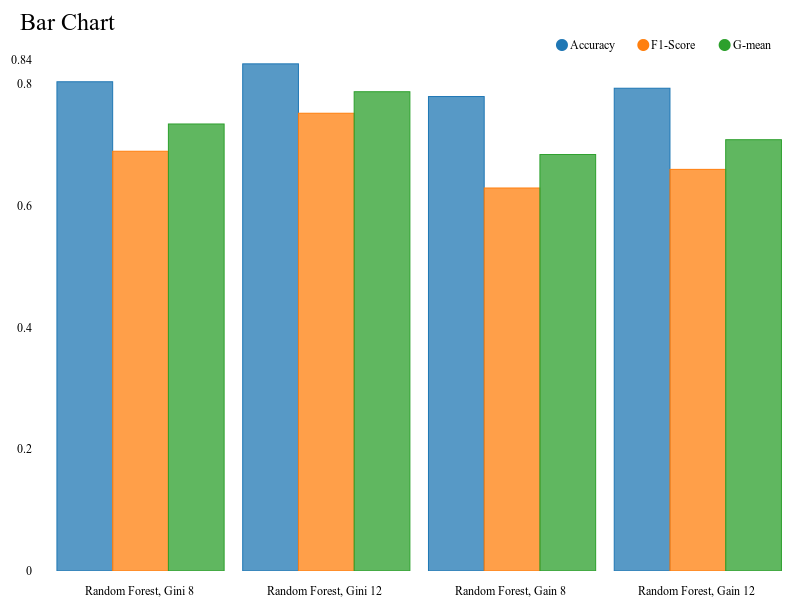
\includegraphics[width=0.87\textwidth]{img/rfcom.png}
		\caption{Gráfico de Barras - Random Forest}
	\end{figure}

	
	Mostramos la curva ROC resultante:
	
	\begin{figure}[H]
		\centering
		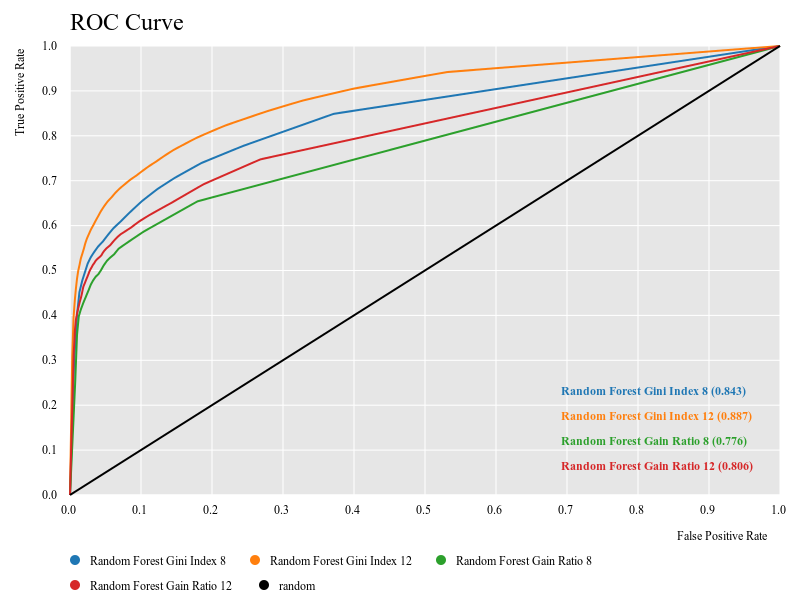
\includegraphics[width=0.87\textwidth]{img/rfroc.png}
		\caption{Curva ROC Random Forest}
	\end{figure}
	
	Se ve claramente que a mayor número de hebras se obtienen mejores resultados, además, \textit{Gini Index} supera a \textit{Gain Ratio} ya que este último añade otro factor que penaliza a los atributos con un gran número de valores distintos, como puede ser el caso.
	
	Si el dominio de las variables de nuestro dataset no fuera tan elevado, los resultados serían más o menos igualados ya que el nº de hebras usadas es bajo, lo que se traduce en una menor diferencia de precisión.
	
	
	Comprobamos el Overfitting de nuestro algoritmo:
	
	\begin{figure}[H]
		\centering
		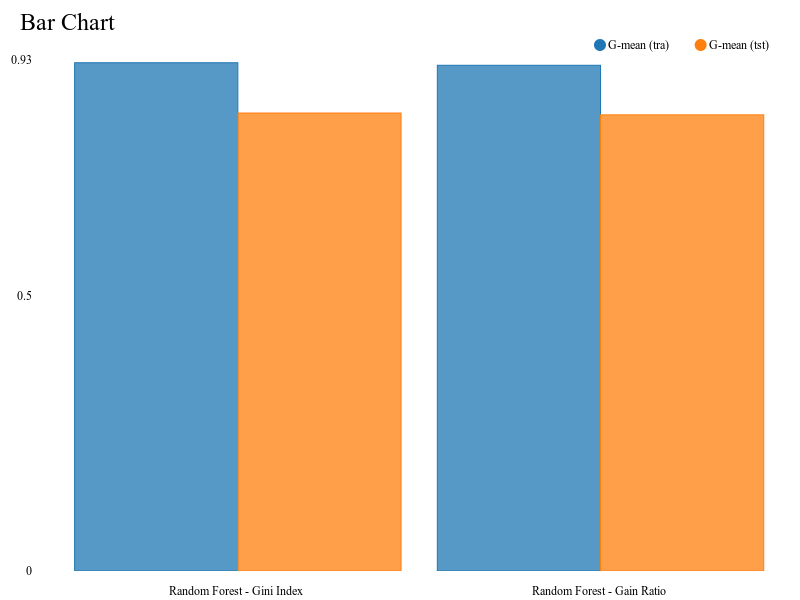
\includegraphics[width=0.7\textwidth]{img/sobrerf.png}
		\caption{Overfitting Random Forest}
	\end{figure}

	Observamos que no existe prácticamente Overfitting en nuestro algoritmo. El G-mean del training es ligeramente superior (como cabe esperar) del G-mean del test, pero esta diferencia es prácticamente nula.

	\subsection{ID3}
	
	\hspace{1cm} ID3 no admite la elección de un parámetro a modificar. Por ello, realizamos un preprocesado básico y sobreentrenamiento para así poder compararlos.
	\begin{figure}[H]
		\centering
		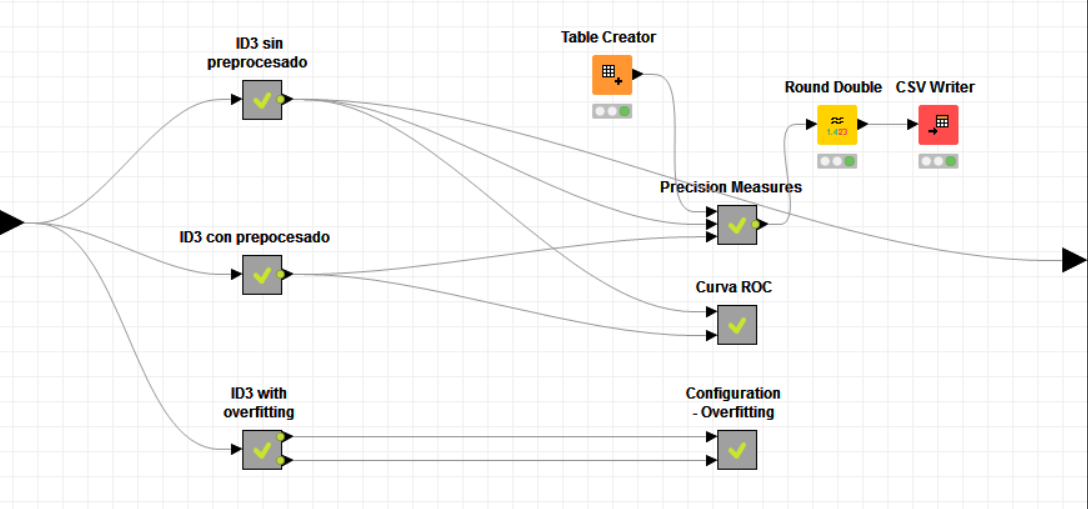
\includegraphics[width=0.8\textwidth]{img/id3comp.png}
		\caption{Comparativa ID3}
	\end{figure}

	La comparativa cumple nuestras expectativas ya que se ha realizado un filtrado de columnas y un \textit{One to Many} de una sola columna. El algoritmo emplea para su construcción árboles y como bien sabemos por teoría, estos usan el criterio de ganancia de información. Por esto, cuando eliminamos columnas se traduce en un mayor error.
	
	Mostramos los resultados de todos los índices y algoritmos en una tabla comparativa:

	\begin{table}[h]
		\resizebox{\textwidth}{!}{%
			\begin{tabular}{|l|l|l|l|l|l|l|l|l|l|l|l|}
				\hline
				\textbf{Algoritmo}               & TP    & FP   & TN    & FN   & TPR   & TNR   & PPV   & Accuracy & F1-Score & G-mean & AUC \\ \hline
				\textbf{ID3 sin preprocesado} & 15995 & 3694 & 32882 & 6829 & 0.701 & 0.899 & 0.812 & 0.823    & 0.752    & 0.794  & 0.853            \\ \hline
				\textbf{ID3 con preprocesado} & 15273 & 3453 & 33123 & 7551 & 0.669 & 0.906 & 0.816 & 0.815    & 0.735    & 0.778  & 0.849            \\ \hline
			\end{tabular}%
		}
	\end{table}


	Representamos ahora en una curva ROC el AUC tanto del ID3 con preprocesado como sin él y vemos que se cumple exactamente lo comentado anteriormente.

	\begin{figure}[H]
		\centering
		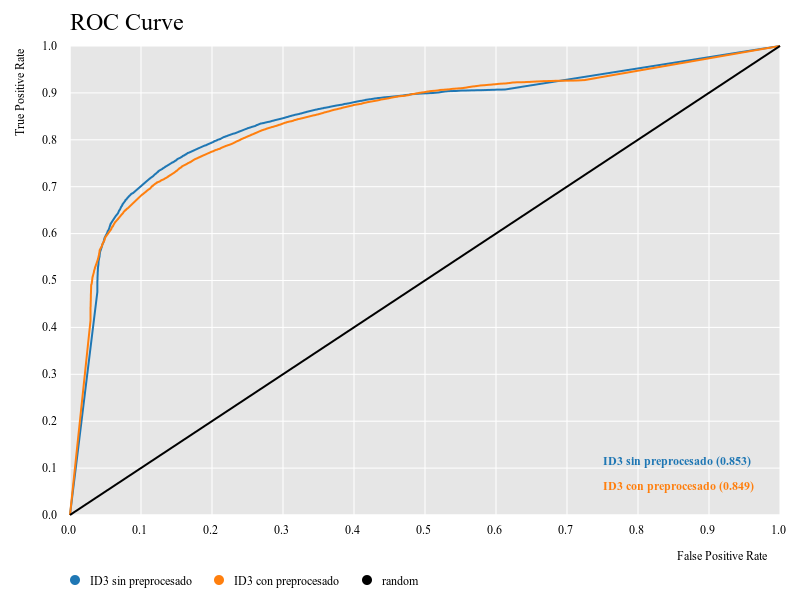
\includegraphics[width=0.9\textwidth]{img/id3roc.png}
		\caption{Curva ROC ID3}
	\end{figure}


	\newpage

	Comprobamos el Overfitting de nuestro algoritmo:
	
	\begin{figure}[H]
		\centering
		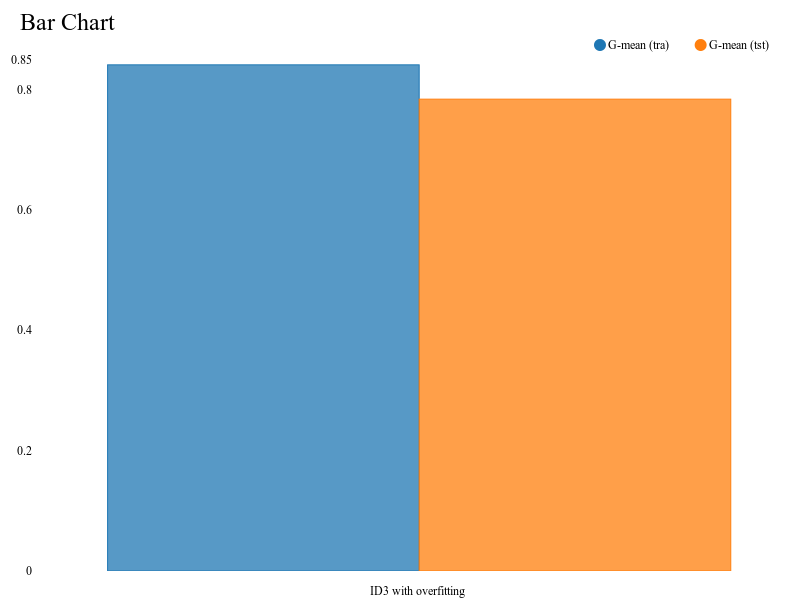
\includegraphics[width=0.65\textwidth]{img/sobreid3.png}
		\caption{Overfitting ID3}
	\end{figure}

	Podemos asegurar que prácticamente no existe Overfitting, la diferencia entre el cociente de ambas medias geométricas es 0.05 por lo que el flujo de trabajo y los nodos usados para el algoritmo son buenos.

	\subsection{C4.5}
	
	\hspace{1cm} Mostramos la estructura del metanodo C4.5
	En esta, separamos entre sobreajuste y no sobreajuste, en el que se realizan distintas modificaciones con sus respectivas tablas.
	
	\begin{figure}[H]
		\centering
		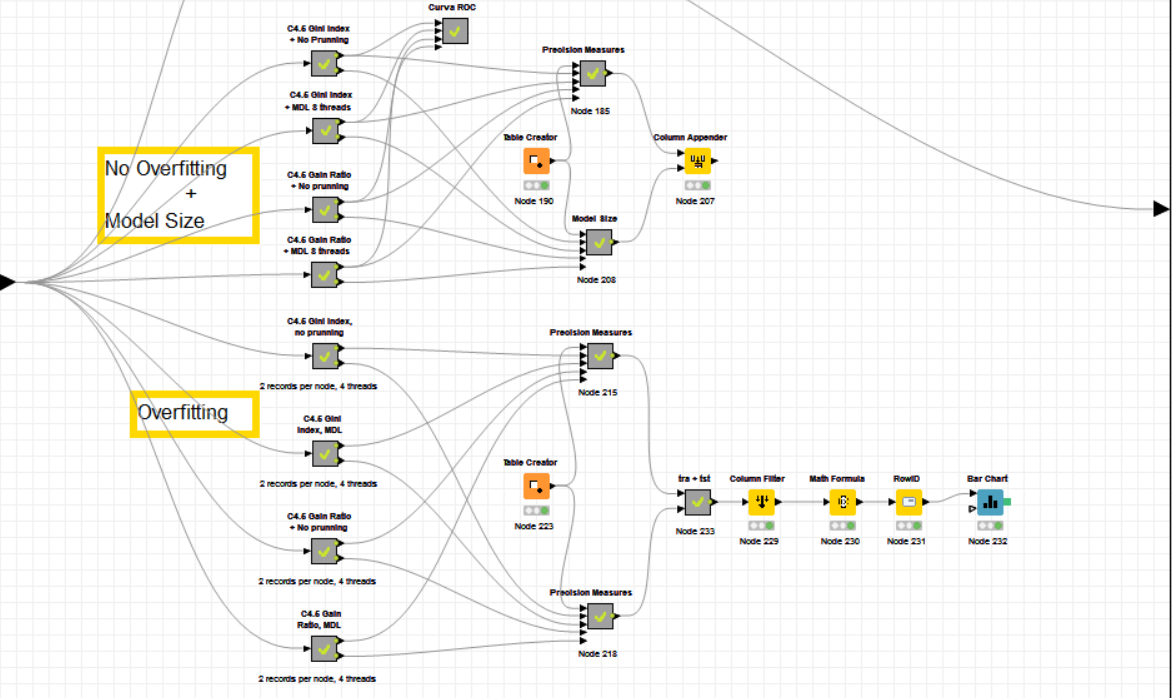
\includegraphics[width=1\textwidth]{img/c45comp.png}
		\caption{Workflow metanodo C4.5}
	\end{figure}


	Mostramos los resultados obtenidos diferenciando entre el criterio de Gini y de Gain Ratio previamente explicados. Además, incorporamos la opción de poda y el tamaño del árbol. Como es normal, en configuraciones con poda se produce un árbol con un menor tamaño mientras que cuando no se poda el tamaño es bastante mayor, lo que supone un mayor tiempo de ejecución y un resultado levemente mejor.

	
	Mostramos la curva ROC asociada. Vemos que el criterio de Gini Index con 8 hebras es claramente superior al resto.

	\begin{table}[H]
		\resizebox{\textwidth}{!}{%
			\begin{tabular}{|l|l|l|l|l|l|l|l|l|l|l|l|l|}
				\hline
				\textbf{Algoritmo}                          & \textbf{TP} & \textbf{FP} & \textbf{TN} & \textbf{FN} & \textbf{TPR} & \textbf{TNR} & \textbf{PPV} & \textbf{Accuracy} & \textbf{F1-Score} & \textbf{G-mean} & \textbf{AUC} & \textbf{Model Size} \\ \hline
				\textbf{C4.5 Gini + No Prunning}         & 17554       & 4950        & 31324       & 5070        & 0.776        & 0.864        & 0.78         & 0.83              & 0.778             & 0.819           & 0.842                     & 7008.8     \\ \hline
				\textbf{C4.5 Gini + MDL 8threads}        & 16242       & 3649        & 32927       & 6582        & 0.712        & 0.9          & 0.817        & 0.828             & 0.76              & 0.8             & 0.873                     & 1134.8     \\ \hline
				\textbf{C4.5 Gain Ratio + No prunning}   & 17354       & 5205        & 31190       & 5345        & 0.765        & 0.857        & 0.769        & 0.821             & 0.767             & 0.809           & 0.826                     & 7760.2     \\ \hline
				\textbf{C4.5 Gain Ratio + MDL 8 threads} & 14713       & 2895        & 33681       & 8111        & 0.645        & 0.921        & 0.836        & 0.815             & 0.728             & 0.77            & 0.842                     & 918.2      \\ \hline
			\end{tabular}%
		}
	\end{table}


	\begin{figure}[H]
		\centering
		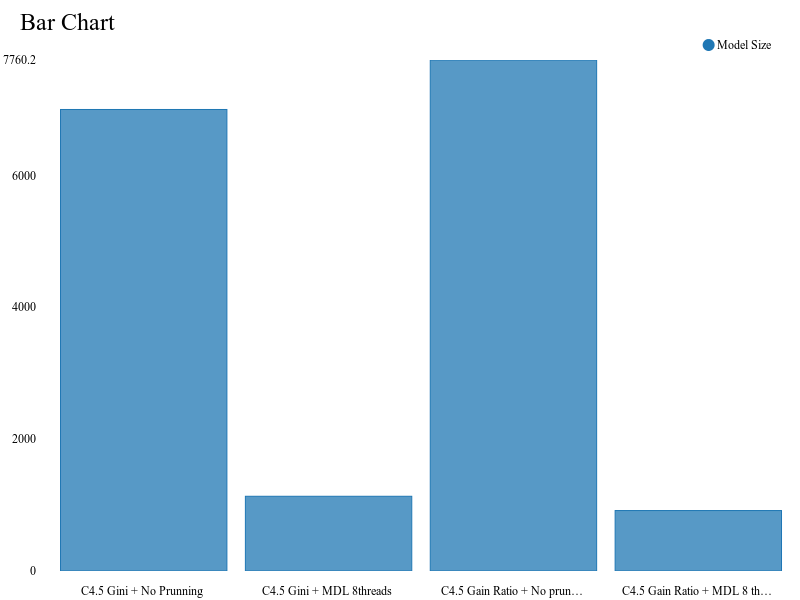
\includegraphics[width=1\textwidth]{img/c45size.png}
		\caption{Model Size C4.5}
	\end{figure}


Mostramos a continuación un gráfico comparativo de los 4 algoritmos en el que se comparan el tamaño del árbol. Como era de esperar, cuando en el árbol se le índica la opción de poda, se reduce consideradamente su tamaño. Por el contrario, cuando no hay opción de poda el tamaño se dispara, independientemente del criterio Gini Index o Gain Ratio usado.

	\newpage 
	Mostramos la curva ROC global:



	\begin{figure}[H]
		\centering
		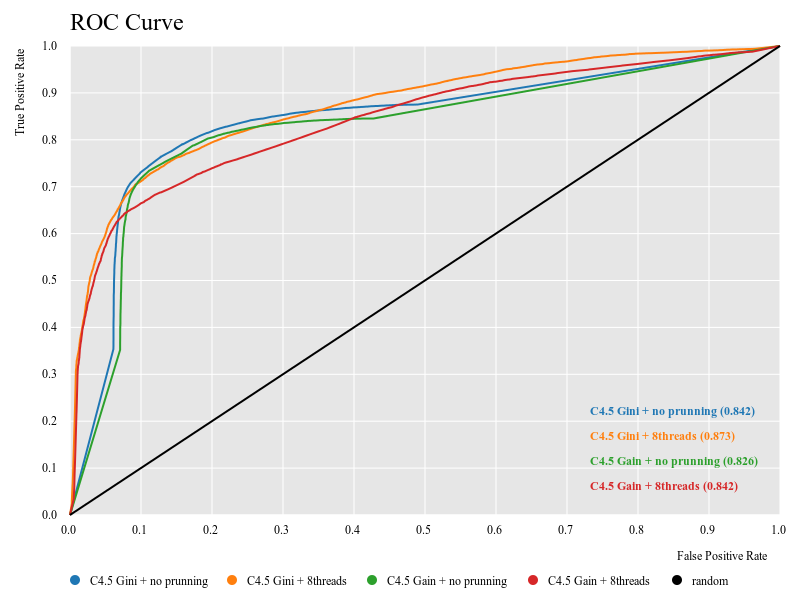
\includegraphics[width=1\textwidth]{img/roc45.png}
		\caption{Curva ROC C4.5}
	\end{figure}


	
	Comprobamos el Overfitting de nuestro algoritmo:
	
	\begin{figure}[H]
		\centering
		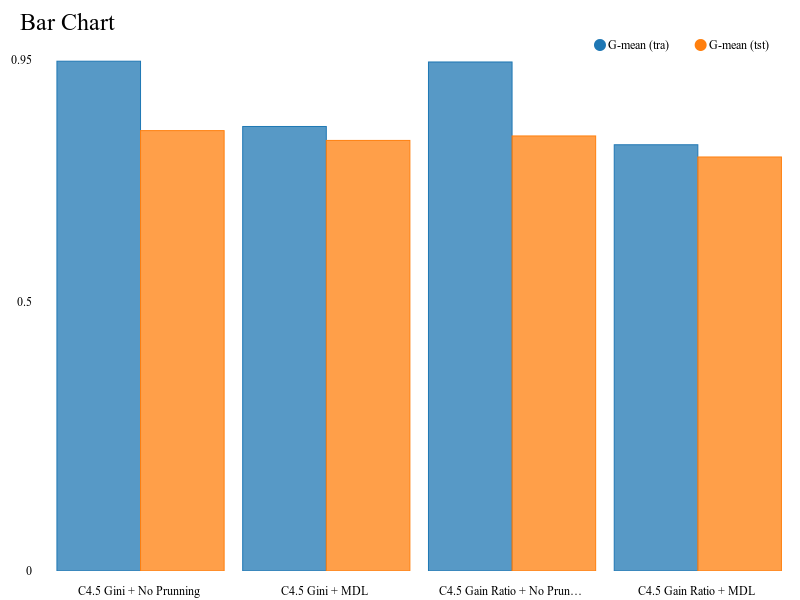
\includegraphics[width=0.7\textwidth]{img/sobrec45.png}
		\caption{Overfitting C4.5}
	\end{figure}

	\newpage
	Observando el gráfico comparativo anterior podemos sacar las siguiente conclusiones:
	\begin{itemize}
		\item \textbf{Prunning}: Cuando hay poda en nuestro algoritmo se reduce el Overfitting. Esto es porque desechamos aquellas ramas que no nos aportan información. Además se reduce el tamaño del árbol y se disminuye el tiempo de ejecución.
		
		\item \textbf{No Prunning}: Cuando no hay poda el overfitting se dispara el Overfitting. No desechamos las ramas que no nos aportan información, lo que se traduce en un mayor ruido, mayor tamaño del árbol y tiempo de ejecución.
	\end{itemize}



	\subsection{KNN}
	
	\hspace{1cm} Hemos realizado un total de 8 configuraciones distintas, 4 con overfitting y otras 4 sin ello.
	Mostramos a continuación los resultados obtenidos:
	
	\begin{figure}[H]
		\centering
		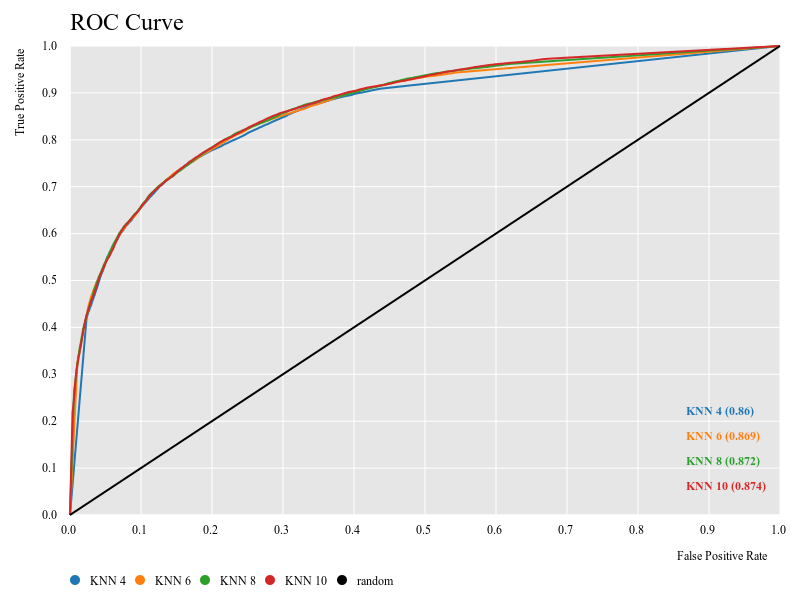
\includegraphics[width=1\textwidth]{img/rocknn.png}
		\caption{Curva ROC parámetros KNN}
	\end{figure}
	
	
	Observando la Curva ROC y la tabla simultáneamente, podemos pensar que a mayor K se obtienen mejores resultados, como es el caso del \textbf{Acuraccy} y de \textbf{AUC}. Sin embargo, observando el resto de parámetros como por ejemplo la media geométrica, KNN=4 es superior al resto. Por lo que podemos asegurar que no hay un claro vencedor y la elección de la K no influye en nuestro dataset.
	
	Realmente, la elección de la \textbf{K} depende fundamentalmente de los datos; generalmente, valores grandes de k reducen el efecto de ruido de la clasificación . 
	Obtenemos los siguientes resultados:
	
	\begin{table}[H]
		\resizebox{\textwidth}{!}{%
			\begin{tabular}{|l|l|l|l|l|l|l|l|l|l|l|l|}
				\hline
				\textbf{Algoritmo} & \textbf{TP} & \textbf{FP} & \textbf{TN} & \textbf{FN} & \textbf{TPR} & \textbf{TNR} & \textbf{PPV} & \textbf{Accuracy} & \textbf{F1-Score} & \textbf{G-mean} & \textbf{AUC} \\ \hline
				\textbf{KNN 4}  & 16560       & 5374        & 31202       & 6264        & 0.726        & 0.853        & 0.755        & 0.804             & 0.74              & 0.787           & 0.86                      \\ \hline
				\textbf{KNN 6}  & 16458       & 5210        & 31366       & 6366        & 0.721        & 0.858        & 0.76         & 0.805             & 0.74              & 0.786           & 0.869                     \\ \hline
				\textbf{KNN 8}  & 16388       & 5086        & 31490       & 6436        & 0.718        & 0.861        & 0.763        & 0.806             & 0.74              & 0.786           & 0.872                     \\ \hline
				\textbf{KNN 10} & 16327       & 5024        & 31552       & 6497        & 0.715        & 0.863        & 0.765        & 0.806             & 0.739             & 0.786           & 0.874                     \\ \hline
			\end{tabular}%
		}
	\end{table}

	Generamos un gráfico \textit{Parallel} y obtenemos: 

	\begin{figure}[H]
		\centering
		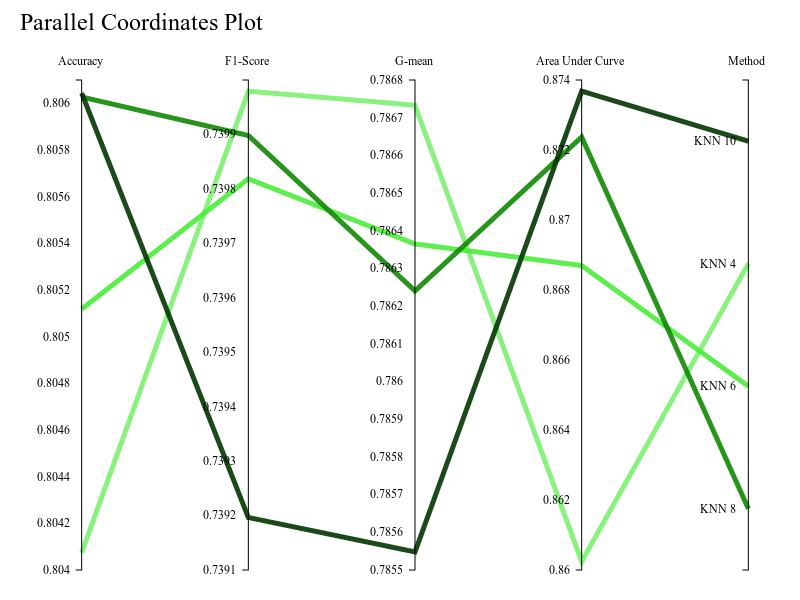
\includegraphics[width=1\textwidth]{img/plotknn.png}
		\caption{Gráfico Parallel KNN}
	\end{figure}

	Aunque parezca que los valores están alocados (ya que se producen muchos picos) todos se mueven en un intervalos pequeño. Sin embargo, hay fluctuaciones, es decir, alti bajos para todos las modificaciones del algoritmo menos con KNN=6. Luego como es la modificación más estable y que ofrece los mejores resultados de media, nos quedamos con esta. \\


	\newpage
	Comprobamos el Overfitting de nuestro algoritmo:
	
	\begin{figure}[H]
		\centering
		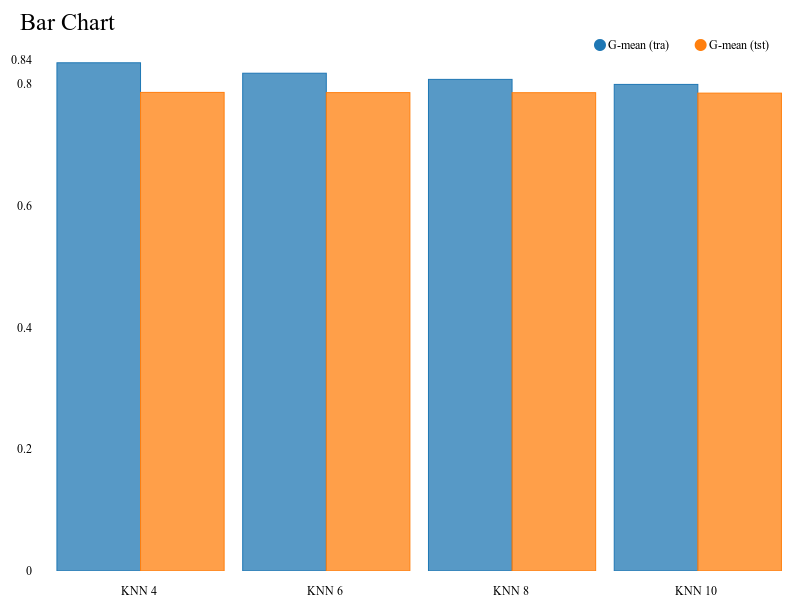
\includegraphics[width=0.7\textwidth]{img/sobreknn.png}
		\caption{Overfitting KNN}
	\end{figure}

	Nos existe prácticamente Overfitting en ninguna de las configuraciones anteriores. Pero si nos fijamos bien, a mayor KNN menor es la diferencia de este. Por lo que reforzamos la explicación anterior y nos quedamos con KNN=6.

	\subsection{Gradient Boosted}
	
	\hspace{1cm} Mostramos la curva ROC obtenida tras ejecutar todas las modificaciones del Gradient Boosted. Estas modificaciones las podíamos haber hecho con el nº de árboles o con la tasa de aprendizaje (learning rate), que controla el grado en que a cada árbol se le permite corregir los errores de los árboles anteriores. 
	
	En nuestro caso, fijamos la tasa de aprendizaje a 0.1 y hacemos variar el nº de árboles. Estos dos parámetros están altamente interconectados en el sentido de que si bajamos el valor en la tasa de aprendizaje vamos a necesitar un nº mayor de árboles para construir un modelo de complejidad similar. Para problemas de gran escala, el rendimiento se podría optimizar usando el algoritmo \textbf{XGBoost}, pero por problemas de pila y características del ordenador donde realizo las comparaciones no hemos podido sacarle gran provecho. \\
	
	\newpage 
	Mostramos la curva ROC global de Gradient Boosted:
	\begin{figure}[H]
	\centering
	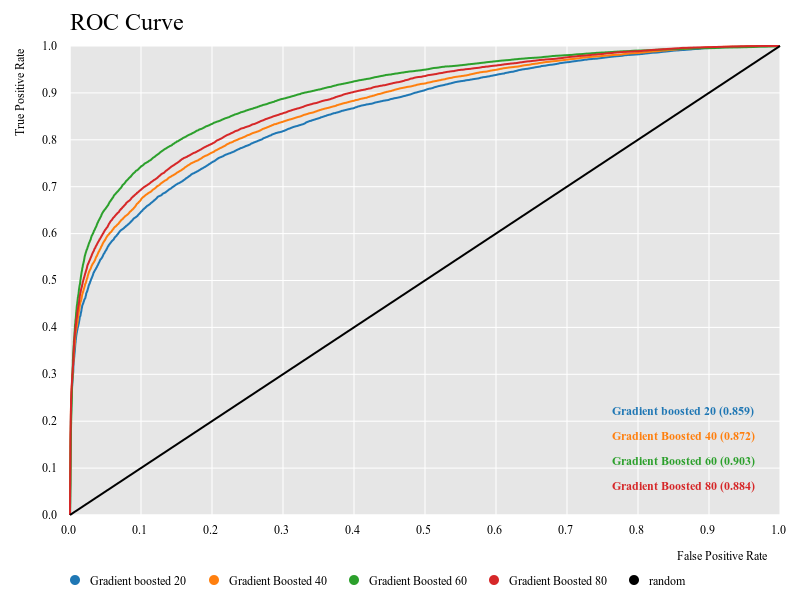
\includegraphics[width=0.87\textwidth]{img/gball.png}
	\caption{Curva ROC parámetros Gradient Boosted}
	\end{figure}	


	Viendo los resultados de la la curva ROC y la tabla de abajo, podemos asegurar que a mayor nº de modelos se obtienen mejores resultados hasta cierto umbral. De hecho, con un total de 60 árboles se obtienen mejores resultados. Además, a mayor nº de árboles se necesita una mayor memoria y tiempo.

	\begin{table}[H]
		\resizebox{\textwidth}{!}{%
			\begin{tabular}{|l|l|l|l|l|l|l|l|l|l|l|l|}
				\hline
				\textbf{Algoritmo}              & \textbf{TP} & \textbf{FP} & \textbf{TN} & \textbf{FN} & \textbf{TPR} & \textbf{TNR} & \textbf{PPV} & \textbf{Accuracy} & \textbf{F1-Score} & \textbf{G-mean} & \textbf{AUC} \\ \hline
				\textbf{Gradient Boosted 20} & 13426       & 2287        & 34289       & 9398        & 0.588        & 0.937        & 0.854        & 0.803             & 0.697             & 0.743           & 0.859                     \\ \hline
				\textbf{Gradient Boosted 40} & 14606       & 2907        & 33669       & 8218        & 0.64         & 0.921        & 0.834        & 0.813             & 0.724             & 0.768           & 0.872                     \\ \hline
				\textbf{Gradient Boosted 60} & 16929       & 3702        & 32874       & 5895        & 0.742        & 0.899        & 0.821        & 0.838             & 0.779             & 0.816           & 0.903                     \\ \hline
				\textbf{Gradient Boosted 80} & 15463       & 3255        & 33321       & 7361        & 0.677        & 0.911        & 0.826        & 0.821             & 0.744             & 0.786           & 0.884                     \\ \hline
			\end{tabular}%
		}
	\end{table}


	\newpage 
	Mostramos de nuevo un grafo \textit{Parallel}. Reforzamos la explicación de que con 60 árboles se obtienen los mejores resultados muy por encima del resto.


	\begin{figure}[H]
		\centering
		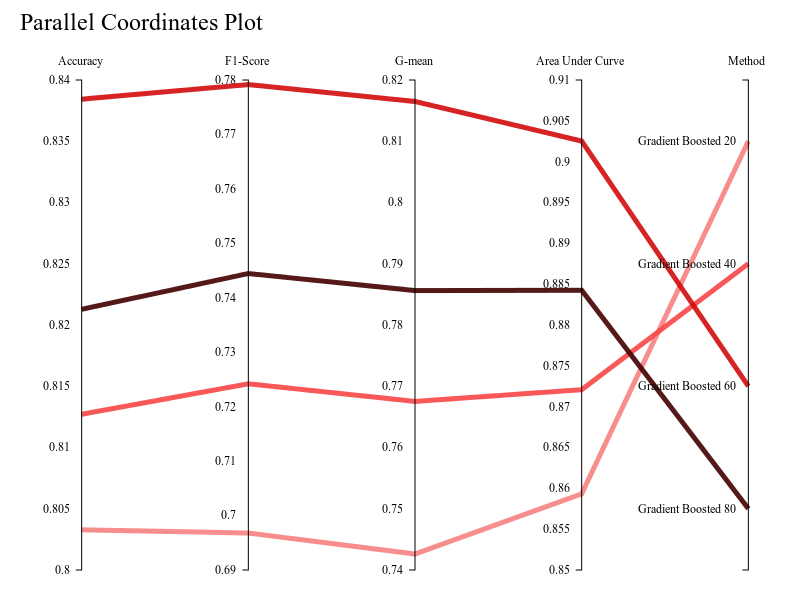
\includegraphics[width=0.8\textwidth]{img/plotgb.png}
		\caption{Gráfico Parallel Gradient Boosted}
	\end{figure}

	Viendo la tabla comparativa del Overfitting anterior podemos asegurar que hasta un uso de 60 árboles no existe practicamente Overfitting pero con Gradient Boosted 80 se produce una diferencia mayor que con el resto. Es por esto por lo que descartamos la modificación de 80 árboles ya que se producen peores resultado, el tiempo de ejecución es mayor y el Overfitting también


	Comprobamos el Overfitting de nuestro algoritmo:
	
	\begin{figure}[H]
		\centering
		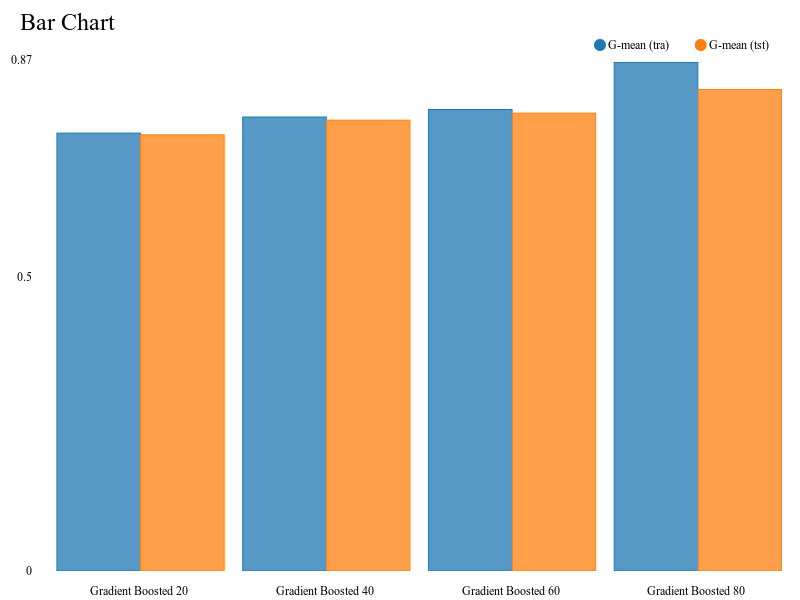
\includegraphics[width=0.7\textwidth]{img/sobregb.png}
		\caption{Overfitting Gradient Boosted}
	\end{figure}

	\subsection{Neural Network}
	
	\hspace{1cm} Ejecutamos las distintas modificaciones variando el nº de iteraciones las cuales se usan para entrenar la red. En nuestro ejemplo probamos desde 50 hasta 200, con saltos de 50 iteraciones. Podemos asegurar que a mayor nº de iteraciones se obtienen mejores resultados. Esto es 'lógico' ya que nuestro modelo se encuentra más entrenado. Sin embargo, si probasemos con más iteraciones nuestro modelo no mejoraría mucho más, ya que la diferencia entre los resultados de cualquier índice se reduce al aumentar dichas iteraciones. Es decir, tomando por ejemplo el área de la curva, la diferencia obtenida entre 200 y 150 es menor que entre 100 y 50. Esto es porque existe un error máximo tolerado que mientras no se haya alcanzado continuará entrenando. \\
	
	Mostramos la curva ROC:
	\begin{figure}[H]
		\centering
		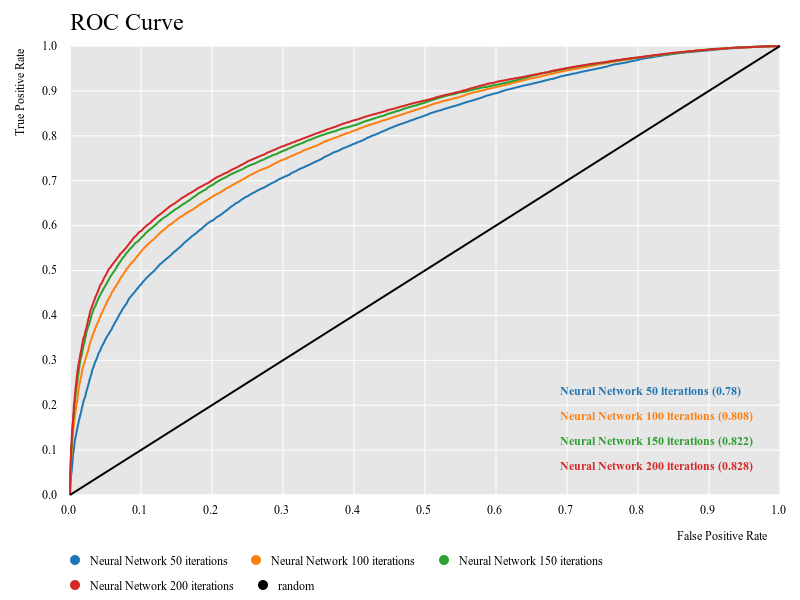
\includegraphics[width=1\textwidth]{img/nnall.png}
		\caption{Curva ROC parámetros Neural Network}
	\end{figure}
	
	Los resultados se corresponden con lo esperado y ya comentado anteriormente, a mayor entrenamiento de la red neuronal, mejores resultados.
	\begin{table}[h]
		\resizebox{\textwidth}{!}{%
			\begin{tabular}{|l|l|l|l|l|l|l|l|l|l|l|l|}
				\hline
				\textbf{Algoritmo}                         & \textbf{TP} & \textbf{FP} & \textbf{TN} & \textbf{FN} & \textbf{TPR} & \textbf{TNR} & \textbf{PPV} & \textbf{Accuracy} & \textbf{F1-Score} & \textbf{G-mean} & \textbf{AUC} \\ \hline
				\textbf{Neural network, 50 iterations}  & 13178       & 6377        & 30199       & 9646        & 0.577        & 0.826        & 0.674        & 0.73              & 0.622             & 0.69            & 0.78                      \\ \hline
				\textbf{Neural network, 100 iterations} & 13991       & 5566        & 31010       & 8833        & 0.613        & 0.848        & 0.715        & 0.758             & 0.66              & 0.721           & 0.808                     \\ \hline
				\textbf{Neural network, 150 iterations} & 14310       & 5189        & 31387       & 8514        & 0.627        & 0.858        & 0.734        & 0.769             & 0.676             & 0.734           & 0.822                     \\ \hline
				\textbf{Neural network, 200 iterations} & 14591       & 5087        & 31489       & 8233        & 0.639        & 0.861        & 0.741        & 0.776             & 0.687             & 0.742           & 0.828                     \\ \hline
			\end{tabular}%
		}
	\end{table}


	\begin{figure}[H]
		\centering
		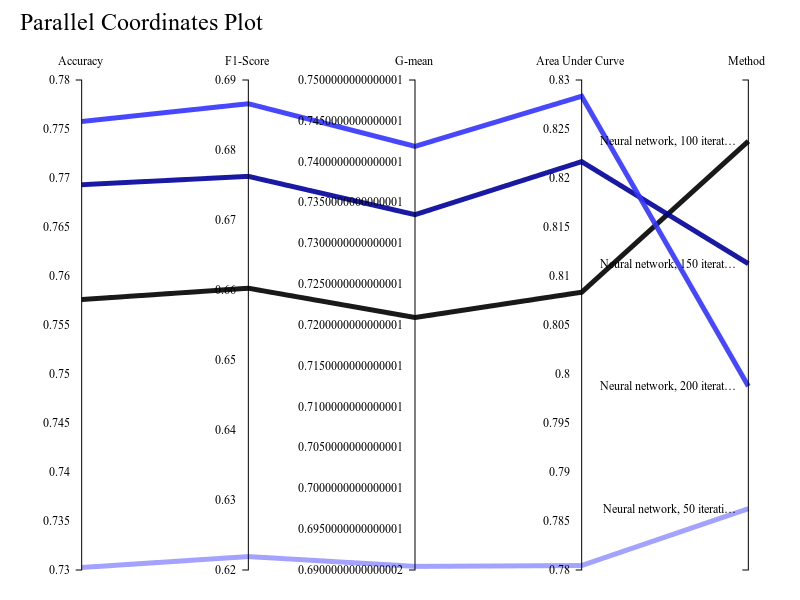
\includegraphics[width=1\textwidth]{img/plotnn.png}
		\caption{Gráfico Parallel Neural Network}
	\end{figure}

	Vemos que el mejor resultado se obtiene con Neural Network 200 iteraciones. Esto es porque nustro algoritmo está más entrenado que con el resto. Sin embargo, se queda bastante por debajo en comparación con los otros algoritmos probados.

	\section{Procesado de datos}
	
	\hspace{1cm} Cabe destacar que todos los preprocesador realizados se han encapsulado en un metanodo llamado \textbf{Estudio de preprocesado de múltiples algoritmos}.
			
	\subsection{Linear Correlation Filter preprocessing}
	
	\hspace{1cm} Preprocesado que consiste en quedarnos con aquellas columnas con mayor correlación entre sí, obviando con \textit{Column Filter} aquellas que tengan menor correlación. 
	
	
	\begin{figure}[H]
		\centering
		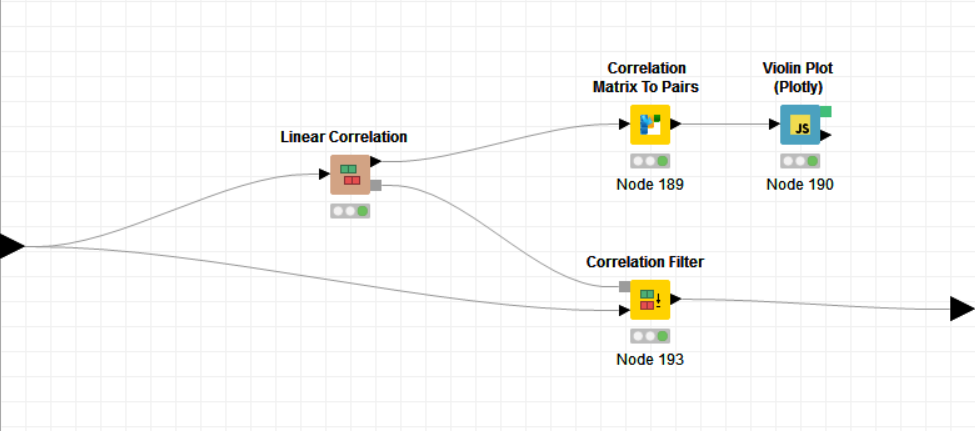
\includegraphics[width=1\textwidth]{img/linear.png}
		\caption{Linear Correlation Filter}
	\end{figure}
	
	
	Para ello usamos el nodo \textit{Linear Correlation} donde previamente hemos tenido que convertir los valores nominales en numéricos. Una vez aquí, filtramos las columnas y nos quedamos con las mejores (en el sentido de mayormente correladas).
	

	\begin{figure}[H]
		\centering
		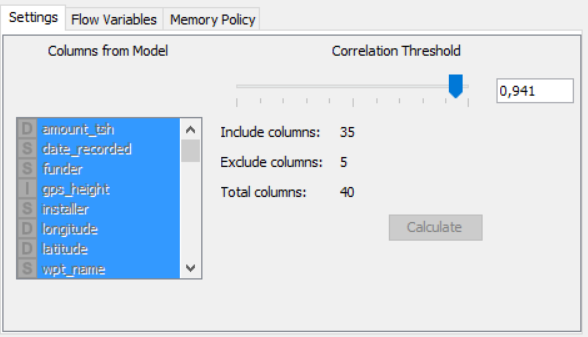
\includegraphics[width=0.75\textwidth]{img/correla.png}
		\caption{Configuración Correlation Filter}
	\end{figure}



	

	Como vemos en la imagen anterior, excluímos 5 columnas y probamos con C4.5 y KNN obteniendo los resultados:
	
	\begin{table}[h]
		\resizebox{\textwidth}{!}{%
			\begin{tabular}{|l|l|l|l|l|l|l|l|l|l|l|l|}
				\hline
				\textbf{Algoritmo}               & \textbf{TP} & \textbf{FP} & \textbf{TN} & \textbf{FN} & \textbf{TPR} & \textbf{TNR} & \textbf{PPV} & \textbf{Accuracy} & \textbf{F1-Score} & \textbf{G-mean} & \textbf{AUC} \\ \hline
				\textbf{C4.5 preprocessed}    & 17544       & 4947        & 31316       & 5067        & 0.776        & 0.864        & 0.78         & 0.83              & 0.778             & 0.819           & 0.842                     \\ \hline
				\textbf{C4.5 sin preprocesar} & 17554       & 4950        & 31324       & 5070        & 0.776        & 0.864        & 0.78         & 0.83              & 0.778             & 0.819           & 0.842                     \\ \hline
				\textbf{KNN preprocessed}     & 16182       & 5723        & 30853       & 6642        & 0.709        & 0.844        & 0.739        & 0.792             & 0.724             & 0.773           & 0.85                      \\ \hline
				\textbf{KNN sin preprocesar}  & 16560       & 5374        & 31202       & 6264        & 0.726        & 0.853        & 0.755        & 0.804             & 0.74              & 0.787           & 0.86                      \\ \hline
			\end{tabular}%
		}
	\end{table}

	\newpage 
		Mostramos la curva ROC, ya que como las clases no están balanceadas y preferimos mostrar AUC como mejor índice alternativo:
	
	\begin{figure}[H]
		\centering
		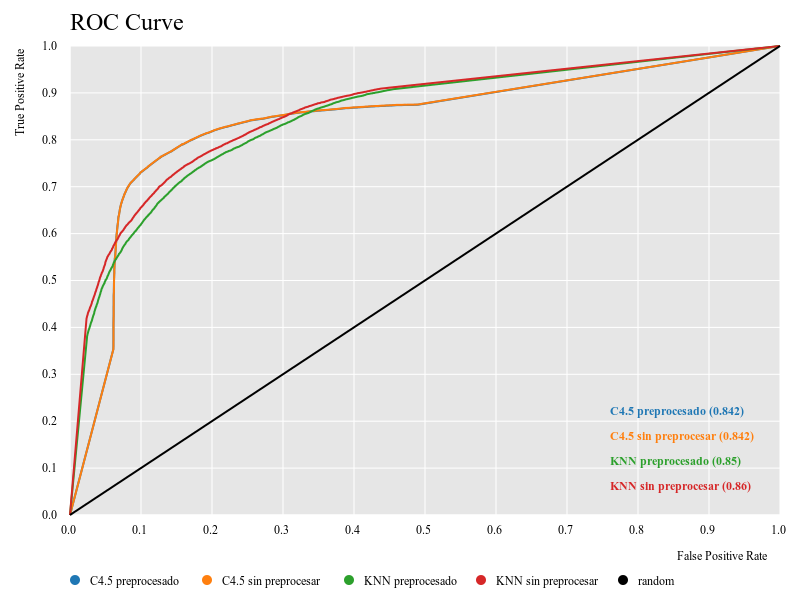
\includegraphics[width=0.75\textwidth]{img/linearroc.png}
		\caption{Configuración Correlation Filter}
	\end{figure}
	
	Observando los resultados tanto de la tabla comparativa como de la curva ROC, vemos que no se ha obtenido una mejora, pues los índices de las distintas medidas de los algoritmos preprocesado son inferiores. 
	
	C4.5 genera un árbol de decisión, que como bien sabemos usa el criterio de ganancia de información. El hecho de quitar columnas se traduce en un mayor error.
	
	Por otro lado, la exactitud de KNN puede ser degradada por la presencia de ruido o características irrelevantes. Mirando la matriz de correlación, hay más de 5 columnas que tienen correlación nula por tanto seguramente si se quitasen un mayor número de variables se podría mejorar el resultado.
	
	\subsection{One To Many preprocessing}
	
	\hspace{1cm} Este tipo de preprocesado toma variables categóricas y te las convierte a numéricas booleanas.
	Se obtiene más precisión si se utiliza en algoritmos en el que normalizan las variables por lo que a priori en algoritmos como KNN debería notarse una cierta mejora. Cuando las variables están normalizadas entre [0,1], ¿realmente nos aporta información relevante que un atributo tenga una probabilidad de 0.5? Para ello usamos el nodo el preprocesado One to Many, donde trabajará con variables numéricas booleanas, que aportan más información.
	
	
	Se deben filtrar las variables cuyo dominio tengan un cardinal bajo, ya que se creará una columna por valor distinto. En este caso hemos seleccionado 3 variables distintas, aunque se deberían haber tomado algunas más. Sin embargo, hay que tener en cuenta que el número de variables tomadas es directamente proporcional al tiempo de ejecución.
	
	
	
	\begin{figure}[H]
		\centering
		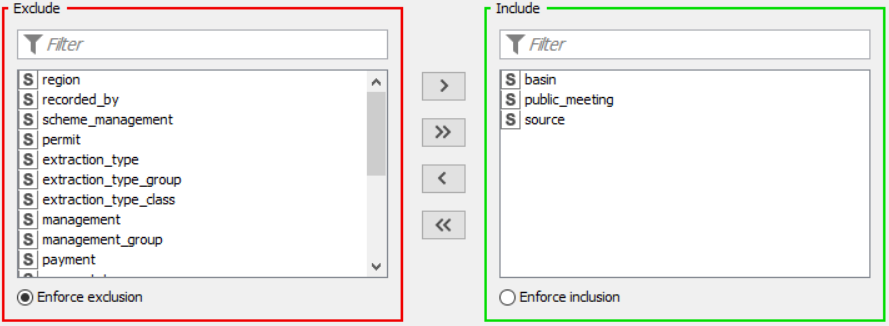
\includegraphics[width=0.7\textwidth]{img/onetomany.png}
		\caption{One To Many Configuration}
	\end{figure}
	
	
	Mostramos los resultados obtenidos tras ejecutar:
	
	\begin{table}[H]
		\resizebox{\textwidth}{!}{%
			\begin{tabular}{|l|l|l|l|l|l|l|l|l|l|l|l|}
				\hline
				\textbf{Algoritmo}               & \textbf{TP} & \textbf{FP} & \textbf{TN} & \textbf{FN} & \textbf{TPR} & \textbf{TNR} & \textbf{PPV} & \textbf{Accuracy} & \textbf{F1-Score} & \textbf{G-mean} & \textbf{AUC} \\ \hline
				\textbf{ID3 sin preprocesado} & 15995       & 3694        & 32882       & 6829        & 0.701        & 0.899        & 0.812        & 0.823             & 0.752             & 0.794           & 0.853                     \\ \hline
				\textbf{ID3 con preprocesado} & 15992       & 3713        & 32863       & 6832        & 0.701        & 0.898        & 0.812        & 0.822             & 0.752             & 0.793           & 0.852                     \\ \hline
				\textbf{KNN sin preprocesado} & 16560       & 5374        & 31202       & 6264        & 0.726        & 0.853        & 0.755        & 0.804             & 0.74              & 0.787           & 0.86                      \\ \hline
				\textbf{KNN con preprocesado} & 16556       & 5407        & 31169       & 6268        & 0.725        & 0.852        & 0.754        & 0.803             & 0.739             & 0.786           & 0.86                      \\ \hline
			\end{tabular}%
		}
	\end{table}

	Ahora, representamos \textbf{Accuracy, G-mean y AUC} en un diagrama de barras:


	\begin{figure}[H]
		\centering
		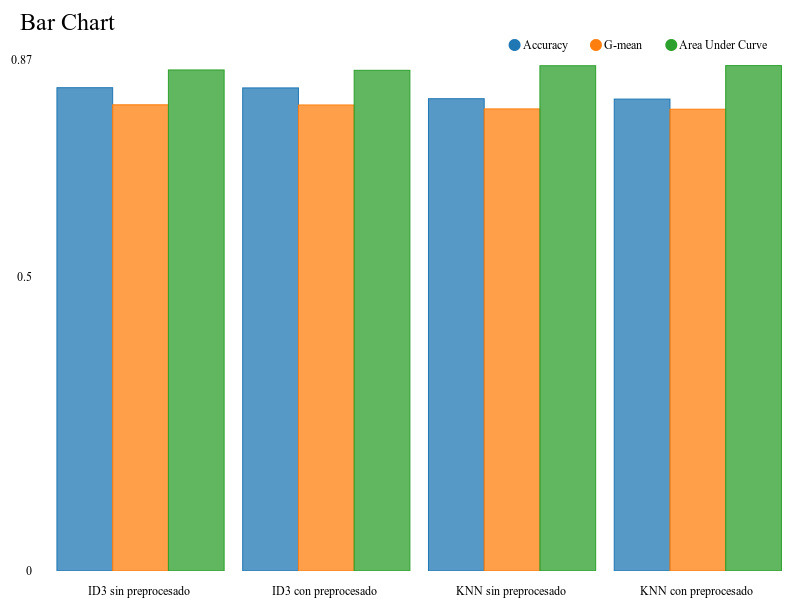
\includegraphics[width=0.8\textwidth]{img/oneto.png}
		\caption{Under Sampling y Over Sampling}
	\end{figure}

	Como observamos y era de esperar, no obtenemos resultados mejores. El algoritmo se mantiene en su línea. Realmente hemos tardado más tiempo en ejecutar para obtener un resultado igual o incluso algo inferior. Si hubiésemos tomado más variables posiblemente se hubiera conseguido una mejor optimización, sin embargo, nuestro ordenador no cumple con unas buenas prestaciones para dicha ejecución.
	
	
	\subsection{Equal Size/Bootstrap preprocessing}
	
	\hspace{1cm} A continuación, realizaremos el último preprocesado de datos realizado en la práctica, conocido como Under Sampling y Over Sampling. Cabe destacar que dicho preprocesado lo consideraremos el mejor realizado ya que los resultados que se obtienen son notablemente mejor.
	
	En Aprendizaje automático este tipo de preprocesado corrige el conocido \textit{Problema de las clases no balanceadas}. Normalmente, los algoritmos traban mejor cuando el número de instancias de cada clase son iguales, es decir, cuando el número de instancias de una clase excede a otra, surgen problemas que se ven reflejados es una peor precisión. 
	
	
	\begin{figure}[H]
		\centering
		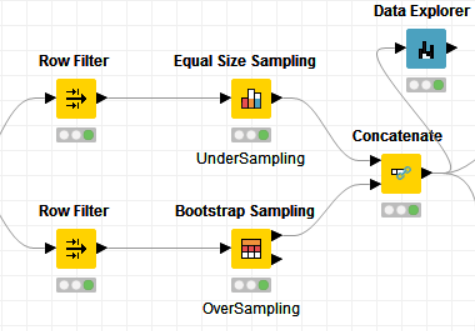
\includegraphics[width=0.6\textwidth]{img/underover.png}
		\caption{Under Sampling y Over Sampling}
	\end{figure}
	
	El primer paso es tomar la clase \textit{Non Functional} y \textit{Functional} y realizar un under sampling con el nodo \textit{Equal Size Sampling}, de este modo, nos quedamos con un total de 23480 instancias.
	
	Por otro lado, realizamos un Over Sampling de la clase \textit{Functional needs repair}, de esta forma nos quedamos con el nº de instancias de la clase intermedia, ya que buscamos un muestreo equilibrado.
	
	Probamos el preprocesado en dos algoritmos, KNN y Neural Network.
	Ejecutamos y obtenemos los siguientes resultados:
	
	\begin{table}[H]
		\resizebox{\textwidth}{!}{%
			\begin{tabular}{|l|l|l|l|l|l|l|l|l|l|l|l|}
				\hline
				\textbf{Algoritmos}                          & \textbf{TP} & \textbf{FP} & \textbf{TN} & \textbf{FN} & \textbf{TPR} & \textbf{TNR} & \textbf{PPV} & \textbf{Accuracy} & \textbf{F1-Score} & \textbf{G-mean} & \textbf{AUC} \\ \hline
				\textbf{KNN sin preprocesar}             & 16560       & 5374        & 31202       & 6264        & 0.726        & 0.853        & 0.755        & 0.804             & 0.74              & 0.787           & 0.86                      \\ \hline
				\textbf{KNN con preprocesado}            & 16702       & 3994        & 41654       & 6122        & 0.732        & 0.913        & 0.807        & 0.852             & 0.768             & 0.817           & 0.901                     \\ \hline
				\textbf{Neural Network sin preprocesado} & 14591       & 5087        & 31489       & 8233        & 0.639        & 0.861        & 0.741        & 0.776             & 0.687             & 0.742           & 0.828                     \\ \hline
				\textbf{Neural Network con preprocesado} & 13944       & 6139        & 39509       & 8880        & 0.611        & 0.866        & 0.694        & 0.781             & 0.65              & 0.727           & 0.815                     \\ \hline
			\end{tabular}%
		}
	\end{table}

	\newpage 
	Haremos uso de \textit{Parallel Coordinates Plot} para ayudarnos a interpretar los resultados:
	
	\begin{figure}[H]
		\centering
		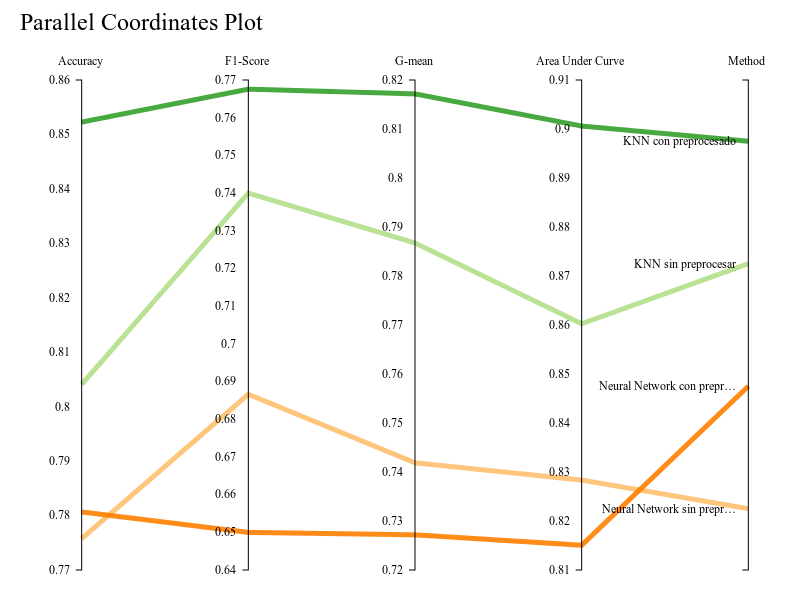
\includegraphics[width=1\textwidth]{img/plotover.png}
		\caption{Under Sampling y Over Sampling}
	\end{figure}
		
	Como podemos observar Neural Network se mantiene. Se incrementa el valor de Accuracy pero decrementan el resto. 
	Por otro lado, el algoritmo KNN con preprocesado mejora bastante, todos los índices mejoran notablemente, desde Accuracy hasta AUC. Así, hemos corregido el problema de las clases no balanceadas y como hemos comprabado, KNN funciona mejor de esta forma.
	
	
		
	\section{Interpretación de resultados}
	
	\hspace{1cm} Por último nos centraremos en los factores que determinan cada clase, es decir qué es lo que influye para clasificar una clase en \textit{functional, non functional o functional needs repair}. Intuitivamente podemos pensar que los factores que determinan su funcionalidad son el clima, ubicación, población total o mantenimiento.
	
	
	
	
	

	
	Para ello, existe un nodo llamado \textit{Linear Correlation} que calcula el coeficiente de correlación de cada par {fila,columna}.
	Así pues, ejecutamos y obtenemos los siguientes resultados:
	
	\begin{figure}[H]
		\centering
		\includegraphics[width=0.8\textwidth]{img/correlation.png}
		\caption{Under Sampling y Over Sampling}
	\end{figure}
	
	Viendo los pares {class, columna} ó {fila, class} (ya que la matriz es simétrica), observamos que la variable que comparte mayor índice de correlación con la clase es \textbf{quantity}, es decir, la cantidad de agua disponible.
	
	
	
	
	
	
	Para el estudio e interpretación de la relación entre estas variables, probamos primeramente con \textit{2D Density Plot}, en el cual compararemos la características que determinan la clase a través de la representación de sus distribuciones en los ejes.
	
	Mostramos los resultados obtenidos tras ejecutar el nodo. Para ello realizamos un pequeño preprocesado (el cual explicaremos más adelante) en el que los datos de entrada tendrán el mismo nº de instancias de cada clase, la intermedia, y así tener la misma probabilidad de coger clases diferentes. Mostramos los resultados obtenidos:
	
	\begin{figure}[H]
		\centering
		\includegraphics[width=1\textwidth]{img/density.png}
		\caption{Preprocesado Sunburst Chart}
	\end{figure}
	
	\begin{itemize}
	
	\item Claramente, cuando la cantidad de agua es suficiente existe una notable tendencia a pertenecer a la clase functional, seguido de functional needs repair.
	\item Si el agua es insuficiente, tiende a ser functional needs repair.
	\item Sin embargo, para el resto de clases no existe una tendencia clara y no podemos establecer una relación class-quantity por lo que procederemos a usar otro gráfico.
	\end{itemize}
	
	
	
	
	
	
	Ahora bien, queremos comprobar la relación de esta variable con \textit{class}, usando \textit{Sunburst Char}. Para ello realizamos el siguiente flujo de trabajo:
	
		\begin{figure}[H]
		\centering
		\includegraphics[width=1\textwidth]{img/igual.png}
		\caption{Preprocesado Sunburst Chart}
	\end{figure}

	Realizamos un pequeño preprocesado, tal y como representamos en la captura anterior. En él, nos quedamos con el nº de instancias de la clase intermedia, es decir, de \textbf{non functional}. Para ello hay que realizar un undersampling de la clase \textbf{functional} y un oversampling de \textbf{functional needs repair} obteniendo un muestreo equilibrado.
	
	Una vez concatenadas las dos tablas, las filtramos para quedarnos con {class y quantity}  y nos quedamos con una muestra de 250 filas cogidas aleatoriamente de la tabla de entrada ya que \textit{Sunburst Chart} no muestra bien los resultados si le pasamos muchas filas.
	
	Mostramos los resultados del gráfico Sunburst:
	
	
	
	\begin{figure}[H]
		\centering
		\includegraphics[width=1\textwidth]{img/sunb.png}
		\caption{Sunburst Chart}
	\end{figure}
	
	
	Haciendo una lectura de la leyenda podemos establecer una biyección entre la clase \textbf{ {functional, non functional, functional needs repair}} y la cantidad de agua disponible en la bomba.
	Por tanto, sacamos las siguientes conclusiones:
	
	\begin{itemize}
		\item \textbf{Enough}: Cuando hay suficiente agua, las bombas pueden a pertenecer a cualquiera de las 3 clases, con una probabilidad aproximadamente del 33\%, inclinándose quizás un poco a la clase functional needs repair.
		\item \textbf{Dry}: Casi el 95\% de las bombas de agua que están secas pertenecen a la clase non functional.
	
		\item \textbf{Unknown}: Cuando no se sabe el estado de \textbf{quantity}, la bomba puede pertenecer tanto a la clase functional como functional needs repair en un 50\%. Com en este caso es imposible representar el 100\% de los datos en el gráfico, podemos prácticamente asegurar que existirá un ligero porcentaje de la clase functional needs repair.
		\item \textbf{Insufficient}: Ocurre exactamente igual que con \textbf{enought}. La tendencia esta vez es hacia la clase functional needs repair, seguido de non functional y por último functional. Esto tiene todo el sentido del mundo, pues si no hay agua en la bomba, la clase seguirá esta proporción usando la lógica.
		
		\item \textbf{Seasonal}: Intuitivamente, cuando tenemos agua temporalmente ocurre igual. En un 50\% de los casos la clase derá del tipo functional needs repair y en otro 50\% aproximadamente pertenecerá a la clase non functional, dejando un pequeño porcentaje a la clase functional.
		
	\end{itemize}

	Para probar que realmente se cumplen estas proporciones, creamos la estructura del árbol de decisión que produce C4.5, pero únicamente con 1 nivel de profundidad pues ver el árbol entero es imposible debido a sus dimensiones. 
	
	\begin{figure}[H]
		\centering
		\includegraphics[width=1\textwidth]{img/tree.png}
		\caption{Árbol de decisión}
	\end{figure}

	Como podemos observar, a partir de la cantidad de agua disponible se le asigna a cada nodo hoja un tipo de clase. Vemos que se forman las siguientes parejas:
	\{enough,functional\}, \{insufficient,functional\}, \{dry,non functional\}, \{seasonal,functional\}, \{unknown,non functional\}, luego se mantiene el porcentage explicado anteriormente.
	
	

	
	
	
	
	
	
	
	
	
	
	
	
	
	
	
	
	
	
	\section{Contenido adicional}
	
	
	\subsection{Filtrado de columnas}
	
	\hspace{1cm} En la ejecución de nuestro algoritmos, hemos encontrado algunas inconsistencias que podemos dividir en dos grupos:
	\begin{itemize}
		\item Warnings: Es una advertencia y no afecta a la ejecución del algoritmo. Normalmente el algoritmo en cuestión ignora columnas por alguna razón (valores perdidos, pérdida de información del dominio...)
		Un ejemplo puede ser en el algoritmo Random Forest o ID3
		
		\item Error: Afecta a la ejecución del algoritmo. No termina.
		Se produce por ejemplo en la Red neuronal.
	\end{itemize} 
	
	Para evitar estas alertas se realiza un filtrado previo a la ejecución de los algoritmos, en este paso, usaremos el nodo \textbf{column filter} en el cual únicamente las columnas seleccionadas pasarán a la tabla de salida.
	
	
	
	\begin{figure}[H]
		\centering
		\includegraphics[width=0.7\textwidth]{img/filtrar.png}
		\caption{Column Filter}
	\end{figure}
	
	
	
	
	\subsection{Datos Perdidos}
	
	\hspace{1cm} Algunos algoritmos usados no trabajan con valores perdidos dando como resultado warnings en la salida de la ejecución. 
	
	\begin{figure}[H]
		\centering
		\includegraphics[width=0.7\textwidth]{img/perdidos.png}
		\caption{Tabla de valores}
	\end{figure}
	
	Por ello, hemos incluído un nodo llamado \textbf{Missing Value } que ayuda a completar todas las celdas en las que se ha encontrado una \textbf{?}, es decir, un valor perdido en la tabla de entrada.
	
	
	\begin{figure}[H]
		\centering
		\includegraphics[width=0.61\textwidth]{img/mean.png}
		\caption{Valores perdidos}
	\end{figure}
	
	Dicho nodo completará los String por el valor más frecuente, ya que es aquel que tiene más posibilidades de ser el valor perdido y todos los números (tanto enteros como de valor real) por la mediana. 
	
	Se han realizado pruebas usando la media en vez de la mediana y se han obtenido resultados mínimamente peores, ya que la media sería una medida buena a usar si los datos fuera homogéneos y no tomasen valores extremos, pero no es el caso, como se muestra a continuación: 
	
	\begin{figure}[H]
		\centering
		\includegraphics[width=.7\textwidth]{img/media.png}
		\caption{Valores extremos}
	\end{figure}
	
	
	\section{Bibliografía}
	
	-Página web de la asignatura:\\
	\href{url}{http://sci2s.ugr.es/graduateCourses/in} \\
	
	-Canal de Youtube del profesor de la asignatura: \\
	\href{url}{https://www.youtube.com/watch?v=NsgY7KJabOg\&t=363s} \\
	\href{url}{https://www.youtube.com/watch?v=OQnfOFlySMM} \\
	\href{url}{https://www.youtube.com/watch?v=wah7TFY933o\&t=477s} \\
	\href{url}{https://www.youtube.com/watch?v=NsgY7KJabOg\&t=423s} \\
	
	
	\newpage
	
	
	
	

		
	\end{document}